\documentclass[12pt]{article}
\usepackage{amsmath}
\usepackage{amsfonts}
\usepackage{bm}
\usepackage[english]{babel} 
\usepackage{xcolor}
\usepackage{textcomp}
\usepackage{graphicx}
\usepackage{natbib} % Powerful citation management
% \usepackage{float}
% \floatplacement{figure}{p}
\bibpunct[; ]{(}{)}{,}{a}{}{;} % Custom minimal bibliography styling
\renewcommand{\baselinestretch}{2}\normalsize
\author{Pierre}
\title{Paper NA}
\date{\today}

\begin{document}

\maketitle

\section{Introduction}

The North American continent consists of an ancient cratonic core, formed during the Archean, that has not been subjected to orogeny for at least 1.8 Ga, bordered to the southeast and east, by progressively younger, stable, Proterozoic provinces \citep{hoffman1988united}. In the west, the Rocky Mountain Front (RMF) separates the Proterozoic and Archean shield from younger, tectonically active provinces (Fig.~\ref{mapgeol}). This relatively regular configuration makes North America an ideal target for seismic tomography, to investigate the relationship of lithospheric and asthenospheric structure to the geological features observed at the surface. 

Differences in the seismic velocity structure between the craton and the western US extending down to at least 200 km were established already in the 1960's and 70's from the first studies of teleseismic P and S wave travel time anomalies  \citep[e.g.][]{cleary1966analysis,herrin1968regional,poupinet1979relation}, the first tomographic images based on P and S travel times \citep{romanowicz1979seismic} and long period surface waveforms \citep{woodhouse1984mapping}, as well as contrasted velocity-depth profiles obtained from the modeling of shear body waveforms at relatively short distances \citep[e.g.][]{grand1984upper}. More recent body wave tomographic models have added considerable details to these images \citep{sigloch2011mantle,burdick2014model,porritt2014seismic,porritt2015lithospheric}

Lateral variations in absolute velocities can be inferred from shear wave tomography, at scales from global \citep[e.g.][]{su1994degree,megnin2000three,shapiro2002monte,panning2006three,kustowski2008anisotropic,ritsema2010s40rts,lekic2011inferring,debayle2012global,schaeffer2013global} to continental \citep{lee2005surface,yuan20113,yuan2014lithospheric,schaeffer2014imaging}. These studies confirm the presence of strong lateral variations in the thickness of the lithosphere across the RMF, with lithospheric roots extending down to 200-250 km under the craton, thinning abruptly to the west to less than 80-100 km. This is also found from azimuthal anisotropy tomography, where  a change in the anisotropy fast axis direction across the lithosphere-asthenosphere boundary (LAB) \citep{marone2007depth,yuan2010lithospheric}.


While the mechanism of craton formation is still widely debated \citep[e.g.][]{s2005archean,lee2011building}, the presence of finer scale lateral and depth variations {\color{red} (cite some body wave tomography studies} in seismic structure suggest a complex history. Moreover, studies of azimuthal anisotropy have shown the presence of laterally varying layering within the cratonic lithosphere \citep[e.g.][]{levin1999shear,deschamps2008stratified,yuan2010lithospheric}, which may indicate different modes and/or times of formation of the top c.a. 100 km of this lithosphere. Fine scale studies of converted and reflected phases indicate the presence of a sharp mid-lithospheric discontinuity (MLD) within the craton, marking the top of a mid-lithospheric low velocity zone \citep{thybo1997seismic,bostock1998mantle,abt2010north,fischer2010lithosphere,rader2015characterization,ford2016midlithospheric} and even possibly several mid-lithospheric discontinuities \citep{calo2016layered}. In addition, there is evidence from radially anisotropic shear wave tomography for separation between blocks of different crustal ages extending to depths of at least 150 km \citep[e.g.][]{yuan2014lithospheric}.


Much of this finer scale structure has been resolved owing to the availability of data from the dense broadband USArray TA deployment. With the completion of the coverage of the conterminous US, as well as availability of data from Canada and Greenland, it is now possible to further refine shear wave tomographic images of North America, and in particular of the stable Proterozoic and Archean provinces, to try and improve our understanding of the different stages of formation of the continent. It is also an unprecedented opportunity to experiment with improved waveform-based tomographic techniques.

In a previous study, we presented a radially anisotropic shear velocity model of the North American upper mantle based on a combination of long period teleseismic and regional waveform data \citep{yuan2014lithospheric}. The regional waveform data (down to 40 s period) were, for the first time at this scale, compared to 3D synthetics computed using RegSEM \citep{cupillard2012regsem}, a Spectral Element Method (SEM) code suitable for continental-scale wavefield computations. Due to the very heavy computations that would have been necessary to compute the predicted teleseismic wavefield numerically at each iteration of the inversion, the latter was, instead, computed using Non-Linear Assymptotic Coupling Theory \citep[NACT,][]{li1995comparison}, a methodology based on normal mode perturbation theory, that is computationally more efficient (albeit approximate), and has been used in the development of several generations of global and continental scale shear velocity models based on time-domain waveform inversion \citep{li1996global,megnin2000three,gung2003global,panning2006three,yuan20113}
 
The resulting 2014 model of North America presents some interesting features, in particular a correlation of radial anisotropy structure with lithospheric blocks corresponding to different orogenies in the eastern US and continental shelf. 
While more rigorous than inversions practiced by most groups and based on the path-average surface wave approximation \citep[PAVA,][]{woodhouse1984mapping}, this mixed methodology nevertheless presents some inconsistencies from the theoretical point of view, since the predicted wavefield through the target model space is computed with different theories for teleseismic and regional distance data, respectively.

 To better integrate teleseismic data into our regional tomographic inversions, we developed a general framework called "Box Tomography"  \citep[see][]{masson2013numerical,masson2016box,masson2017fast}, that allow us to consistently model and invert both teleseismic (i.e. associated with sources or receivers outside of the imaged region) and regional (i.e. associated with sources and receivers within the imaged region) waveform data using accurate numerical methods such as SEM. 
 In Box Tomography, prior to the inversion, the seismic wavefield generated by teleseismic sources is first modeled numerically at the global scale for a given reference 3D model and is recorded at the surface of the region to be imaged. 
 This reference wavefield is then used to construct virtual sources lying at the boundary of the regional modeling domain and reproducing the original wavefield as illustrated in Figure~\ref{injection}. 
 Once the teleseismic sources have been moved (i.e. replaced by virtual sources) within the regional modeling domain, the tomographic inversion can be performed efficiently in a classical manner (i.e. using regional modeling only) as the teleseismic data are accounted for seamlessly thanks to the virtual sources. 
 Related concepts have been proposed to account for teleseismic data in regional imaging (e.g. Wang et al., 2016 Monteiller et al., 2015), however, in these studies the global modeling of the reference wavefield is performed using a faster method that does not account for the effects induced by the 3D structure of the Earth outside the regional modeling domain. In this paper, we present the first application of Box Tomography to continental scale waveform tomography in North America.


\section{Methodology}

Many studies have inverted for continental scale structure, in particular in North America, using fundamental mode and, in some cases, overtone surface wave dispersion data or waveforms observed at teleseismic distances. 
The usual practice is to first consider the best possible global scale tomographic shear wave velocity model, compute predictions of observables in this model using an approximate theory, generally the surface wave path average approximation \citep[e.g.][]{nettles2008radially,bedle2009svelocity,schaeffer2014imaging}, or, in our group, NACT \citep{marone2007three,yuan20113}. 
In the case when secondary observables such as dispersion data are considered, the contribution from outside of the target region is calculated once and for all in the background global model, and subtracted from the observed dispersion data. 
The resulting residual is attributed to structure in the target region and the tomographic inversion proceeds within this target model volume. 
When inverting waveforms, and in particular when a more accurate theory than the PAVA is considered, such a simple procedure is not possible, and it is necessary to recompute the synthetic teleseismic waveforms, at each iteration, in a 3D model which is fixed outside of the target region, and updated only within it. 
This leads to substantial computations, even in the case of an approximate theory such as NACT, and becomes prohibitively expensive, if the 3D teleseismic wavefield is computed using SEM or another accurate numerical method, as especially as one aims to include increasingly shorter periods.

To overcome this problem, we take advantage of the "Box Tomography" theory which allows us to combine teleseismic and regional waveforms in a consistent manner to image regional targets at arbitrary locations. 
This general framework accommodates for arbitrary acquisition setups (i.e. with sources and receivers located outside the regional imaging box), is compatible with most popular numerical methods such as SEM or FD, and can produce exact seismograms and sensitivity kernels (i.e. similar to those obtained when solving the problem globally). 
In this study, we limit ourselves to the situation where both regional and teleseismic events are employed but where all the seismic stations lie within the regional computational domain. 
Furthermore, we neglect some higher order scattering effects, as proposed by \cite{masson2016box}. 
In this situation, Box Tomography is particularly efficient, as the computational effort  to account for teleseismic data in regional inversions is limited to a few global scale simulations that are done once and for all prior to the inversion. \cite{masson2016box} showed that this approach can produce accurate regional tomographic images even though the elastic structure outside the imaged region is neither fully known prior to the inversion, nor updated during the inversion.  

Here, we apply this methodology to the case of teleseismic three component waveform data observed at stations within North America, combined with "regional" waveform data for which both earthquakes and stations are located within the target region. 
This is the first time this methodology is applied in practice, and this study represents a proof of concept for this approach. 
Adding teleseismic data allows better azimuthal coverage of the target region than can be achieved using only the regional dataset, and eventually provides for the inclusion of constraints from additional phases such as, for example, teleseismic SS phases reflected inside the target region.



\subsection{Dataset and model parametrization}.

The dataset includes three component acceleration waveforms from 2860 permanent and temporary broadband stations located in the target region, a $89^o \times 89^o $ area encompassing most of north America (Figure ~\ref{map_evt_stn}). We considered two different datasets:
\begin{itemize}
	\item a regional dataset consisting of 155 events ($4.5 < M_w < 6.0$) for which sources are located within the target region.
	\item a teleseismic dataset, consisting of 122 events ($5.5 <M_w <6.9$) for which sources are located outside of the target region.
\end{itemize}

The waveforms are filtered between 40 and 400 s, with corner frequencies at 53 and 250 s, and windowed into wavepackets, according to the procedure of \cite{li1996global} ,allowing different weights to be applied according to relative amplitude of individual wavepackets, redundancy of paths and signal to noise ratio. 
This weighting step is crucial, as it homogeneizes the data coverage within the region and provides a way to construct the data covariance matrix $C_D$, which we approximate as a diagonal matrix. 
At each iteration of the inversion, only those wavepackets are considered that satisfy predefined goodness of fit criteria compared to synthetics calculated in the current 3D model, in particular to avoid cycle slipping in our time domain waveform inversion procedure. 
As the model improves, at each iteration, additional wavepackets are included. 
The total number of wavepackets of fundamental and overtone Love and Rayleigh waves is given in Table 1, and provides a good coverage within the NA continent (Figure ~\ref{density_coverage}).


In addition to long period waveforms, we also consider a group velocity dispersion dataset \citep{shapiro2002monte} provided in the form of $1^o \times 1^o $ maps between 25 and 100 s. 
The shorter periods (below 60 s) are used to constrain our homogeneized crustal structure at each iteration, as described below, while the entire period range is included during the inversion for mantle structure, providing additional constraints for structure in the shallow parts of the mantle, that are consistent with the treatment of the crust.

As in our previous work at the global scale \citep{french2013waveform,french2014whole}, we do not rely on an existing layered crustal model. 
There are several drawbacks to considering such models. 
First, they are constructed using data for limited regions that are then extrapolated to other regions based on a tectonic regionalization, and may not always fit real waveform data very well. 
Second, the inclusion of thin low velocity layers slows down the SEM computation significantly. 
Instead, we compute a radially anisotropic smooth crustal model on a $2^o \times 2^o $ grid through Monte Carlo Markov Chain (MCMC) simulation constrained by the group velocity dispersion data. 

This process is called "homogeneization" \citep[e.g.][]{backus1962long,capdeville2008shallow}, and yields a crustal model equivalent to a real crust within the period range of the data used to constrain it (i.e. here for periods longer than 20s). 
The thickness of the crust is a priori fixed to that of model Crust2.0 \citep{basscrust2} when it is larger or equal to 30 km, and it is fixed at 30 km in regions where it is thinner. 
This results in a smooth, but realistic crust within most of the continent, and a crustal model that is not directly interpretable in the border regions of our model space (i.e. in the oceans and borders of the continent where the real crust is thin). 
We have shown that this does not bias the mantle structure imaged below 50 km \citep{french2014whole}. 
At each iteration of the inversion, we only invert for structure below 30 km depth, and subsequently recompute the crustal model for the next iteration by applying our MCMC approach with mantle structure fixed to that of the current iteration model. 
The procedure is described and discussed in detail in \cite{french2014whole}

Assuming that our azimuthal coverage is everywhere sufficient within our target region, we here solve only for radially anisotropic structure. If (A,C,F,L and N) are the 5 elastic parameters describing a radially anisotropic (or VTI) medium \citep{love2013treatise}, then:

\begin{equation}
 N = \rho V^{2}_{SH}, \quad L = \rho V^{2}_{SV}, \quad A = \rho V^{2}_{PH} , \quad C = \rho V^{2}_{PV} 
 \end{equation}
then the medium can equivalently be described by the 5 parameters ($V_{S}, V_{P}, \xi, \phi, \varepsilon$) where:

\begin{equation}
V_{S} = \sqrt{\frac{2V^{2}_{SV}+V^{2}_{SH}} {3}} \\
V_{P} = \sqrt{\frac{V^{2}_{PV} + 4V^{2}_{PH}}{5}}
 \xi = \frac{N}{L}, \quad \varphi = \frac{C}{A}, \quad \eta = \frac{F}{A-2L} 
 \end{equation}

We only consider two of the 5 independent anisotropic parameters , those to which long period surface waveforms are the most sensitive: isotropic velocity $V_{S}$ and the anisotropic parameter $\xi = {\frac{V_{SH}}{V_{SV}}}^2$, where $V_{SH}$ is the velocity of waves polarized horizontally and $V_{SV}$ that of waves polarized vertically . 
The other three parameters and density are constrained through empirical scaling relationships, following \cite{montagner1989petrological}, and are based on laboratory measurements for upper mantle rocks. 

The scaling parameters considered are \citep{montagner1989petrological}

 \begin{equation}
\frac{\delta(V_{P})}{\delta(V_{S})} = 0.5, \quad
\frac{\delta(\rho)}{\delta(V_{S})} = 0.33, \quad
\frac{\delta(\eta)}{\delta(\xi)} = -2.5,   \quad
\frac{\delta(\varphi)}{\delta(\xi)} = -1.5,   \quad
\end{equation}

We chose a parametrization in terms of $V_S$ and $\xi$, rather than $V_{SH}$ and $V_{SV}$, as this allows us to consider different spatial resolution and apply higher damping in the inversion to the less well resolved anisotropic parameter $\xi$, rather than having to reconstruct this parameter from differences in perturbations in the two quantities $V_{SH}$ and $V_{SV}$, which would limit the resolution allowed in isotropic velocity.

In previous studies \citep{marone2007depth,yuan2010lithospheric}, after inverting for radial anisotropic structure \citep{marone2007three,yuan20113}, we also inverted for azimuthal anisotropy, by adding constraints from SKS splitting measurements. This step will be the topic of a separate publication.  

The target model space is geographically defined as shown in Figure ~\ref{map_evt_stn}, and is limited in depth down to 800 km. 
As in our previous tomographic studies, the model space is parametrized in terms of 26 cubic splines $\nu_{q}(r)$ vertically \citep{megnin2000three} from the core-mantle boundary to 30 km deep. 
Although we invert for structure only in the top 16 splines, corresponding to the top 700-800 km of the mantle. 
The spline nodes are spaced more closely at shallow depths, and located at the following radii: 5690, 5810, 5910, 5900, 6061, 6101, 6131, 6161, 6191, 6221, 6241, 6261, 6281, 6301, 6321, 6341 km.  
Laterally, we parametrize our model in terms of spherical splines $\beta(\theta,\phi)_{p}$ \citep{wang1995spherical}. 
The combination of vertical and spherical splines constitutes a local basis for the description of smooth functions within the model volume. 
Thus, the value of a model parameter $m(r,\theta,\phi)$ can be computed at any point in space given the set of spline coefficients $m_{pq}$:

\begin{equation}
	m(\theta,\varphi,r) = \sum_{p}\sum_{q}m_{pq}\beta_{p}(\theta,\varphi)\nu_{q}(r)
\end{equation}

The spherical spline parametrization has the advantage of allowing for variable grid parametrization, which can be adjusted according to data coverage \citep[e.g.][]{marone2007three}. 
In our case, outside of the target region, we adopt a "level 6" spherical grid for $V_{S}$ ($2^{o}$ knot spacing) and a "level 4" spherical grid for $\xi$ ($8^{o}$ knot spacing), consistent with the parametrization of $SEMUCB\_wm1$ \citep{french2014whole}. 
Inside the well-sampled target region, we define a level 7 spherical grid ($1^{o}$ knot spacing) for $V_{S}$ and level 6 ($2^{o}$ knot spacing) for $\xi$. 

 \subsection{Forward modelling}

During the inversion, all the synthetic seismograms are computed using the regional SEM code RegSEM \citep{cupillard2012regsem} that takes into account effects of oceans, topography/bathymetry, ellipticity, and anelasticity, and where the limits of the computational domain (white box around North America in Figure~\ref{injection} and red box in Figure ~\ref{map_evt_stn}) are dealt with using absorbing boundaries. 
The synthetic seismograms associated with regional data (i.e. where both the seismic stations and the earthquake are located within the regional modeling domain) do not require any specific treatment and are computed as in our previous studies using RegSEM \citep[e.g.][]{yuan2014lithospheric}. 
The synthetic seismograms associated with teleseismic data (i.e. where the earthquake and the seismic stations are located outside and inside the regional modeling domain, respectively) are obtained using a two step procedure as proposed by \cite{masson2016box} as follows. 

Prior to the inversion, the wavefields generated by teleseismic earthquakes are computed globally within our starting model ($SEMucb\_wm1$) and a version of $SPECFEM3D\_globe$ \citep{komatitsch2002spectrala} adapted to this model representation. 
During these global simulations, the 3 component displacement wavefield is recorded at a set of points with locations prescribed by the RegSEM code.
Within the regional solver RegSEM, these points are the collocation or Gauss-Lobatto-Legendre (GLL) points belonging to the one element thick surface surrounding the regional modeling domain \citep[see][]{masson2013numerical}. 
Note that our procedure does not require to store either the stress or the strain wavefield, which are computed naturally by the regional solver. This makes it easy to swap between different codes for modeling global seismic wave propagation (i.e. any code that outputs displacement seismograms can be used as such).
Because the Courant criteria which ensure the stability in SEM often lead to oversampling, we compress the recordings versus time using a least square B-spline transform \citep{unser1993a,unser1993b}. We found this  approach more efficient and practical than the more classic decimation/interpolation scheme.
We typically achieve a data compression ratio of between 10 and 100 with no significant loss of accuracy. 
During the inversion, the global recordings are transformed to virtual sources that regenerate the global wavefield regionally. 
This operation is done on the fly by the RegSEM code.

Overall, the additional computational effort to account for teleseismic events consists of one global simulation per teleseismic event. These simulations are done once and for all before the inversion starts. A comparison between regular $SPECFEM3D\_globe$ and ``RegSEM + virtual sources`` synthetics is shown in Figure~\ref{injection}.

\subsection{Inverse modelling}

In continuity of our previous work \citep[e.g][]{marone2007three,yuan20113,yuan2014lithospheric}, we use a hybrid iterative inversion scheme where, at each iteration, the forward wavefield is computed accurately using SEM, but the inverse step is solved using the formalism of \cite{tarantola1982generalized} with sensitivity kernels calculated approximately using normal mode perturbation theory. 
This allows us to apply a fast converging Gauss-Newton quadratic optimization scheme. 
As shown in \cite{tarantola2005inverse}, and in Appendix A of \cite{lekic2011inferring}, it is far more important to use an accurate forward modelling scheme to compute the misfit function, provided of course that the theory captures the effects of the background long wavelength structure accurately \citep[unlike the examples shown in][]{valentine2016impact}.
Inaccuracies in the theoretical treatment of kernels then result in smoothing errors that can be compensated for in subsequent iterations. In contrast, currently popular "adjoint tomographic" approaches \citep{zhu2015seismic,bozdag2016global} compute the numerically exact gradient, however, they also need to apply smoothing operators and regularization, which degrades the accuracy of their kernels. Importantly, they rely on a linear optimization scheme (conjugate gradient method), which is characterized by very slow convergence.

Our misfit function is defined in the time domain from the point by point differences between observed and synthetic waveforms as follows:
\begin{equation}
2\Phi(m_{k}) = [d - g(m_{k})]^{T} C^{-1}_{d} [d-g(m_{k})] + [m_{p}-m_{k}]^{T} C_{m}^{-1} [m_{p}-m_{k}]
\end{equation}

\noindent where $m_{k}$ represents the model estimate at the k-th iteration, $d$ is the data vector (waveform discretized in time or group velocity as a function of period) and $g(m_k)$ is the corresponding discretized wavefield computed using SEM, or the predicted group velocity dispersion. The model prior is $m_p$  (i.e. the 3D starting model) and $C_m$ and $C_d$ represent a priori model and data covariance matrices, respectively. Minimizing $\Phi$ in the sense of the L2 norm leads to the equation for the k+1 model update:

\begin{equation}
m_{k+1} = m_{k} + (C_{m}G^{T}_{k}C^{-1}_{d}G_{k} + I)^{-1} (C_{m}G_{k}^{T}C^{-1}[d-g(m_{k})]+ m_{p}-m_{k})
\end{equation}

\noindent where $G$ is the matrix of Frechet derivatives of $g(m)$ calculated at $m_k$. We compute G using NACT or PAVA, depending on the distance range of the corresponding source-station path.
NACT and PAVA are both asymptotic (high frequency) approximations to first order normal mode perturbation theory. 
The PAVA includes along branch mode coupling only and is equivalent to the standard surface wave approximation \citep[e.g][]{mochizuki1986free,romanowicz1987multiplet}, as used for example in \cite{woodhouse1984mapping}, in which a frequency shift and distance shift are introduced for each mode to account for the effects of heterogeneous structure. 
The corresponding kernels are "1D", i.e. they only depend on the average structure between the source and the receiver. This approximation is valid for single-mode seismograms, such as fundamental mode surface waves \citep[e.g][]{romanowicz2008computation}.
NACT includes across branch-coupling, in addition to PAVA, which brings out 2D sensitivity of waveforms in the vertical plane containing the source and the receiver. NACT breaks down when the distance between the source and station is short, so we compute kernels using NACT for epicentral distances larger than $15^o$, and PAVA for shorter distances.
Neither PAVA nor NACT consider off-great circle plane sensitivity (i.e. focusing effects, e.g. \cite{zhou2005finite}). These effects become important for accurate amplitude fitting. With our choice of misfit function, we are first and foremost fitting the phase, and for that, the 2D effects in the vertical plane are dominant, and important especially for overtones, as illustrated in \cite{megnin1999effects,romanowicz2008computation}.


\section{Results}


	The tomographic inversion results for $V_S$ and $\xi$ are presented in figures \ref{3d-VS} and \ref{3d-Xi} respectvely. 
	We divide the model description and interpretation into two parts, focusing first on the continent-wide structure and then, in more detail, on eastern different regions.

	\subsection{Continental model}

		As observed in many other studies, the average isotropic shear velocity $V_S$ in the shallow upper mantle beneath North America (NA) is high compared to the global average, which contains contributions from large oceanic regions (Figure ~\ref{1daverage}). 
		The difference persists until ca. $270 \: km$ depth and then fades away, though, $V_S$ remains slightly higher in NA than in the global average. 
		Compared to the continental average, precambrian provinces like Wyoming, Yavapai, Mazatzal, Great Rhyolites and Grenville are caracterized by slower velocities. 
		The cordillera region shows the slowest velocities, close the global average as for $\xi$. 
		Closer to the center of the continent, region like Slave, T.H.O, Juvenile arcs and orogens (e.g. Wopmay), Superior; show higher velocities with the Slave province caracterized by a positive gradient above $100 \: km$ deep.

		%The global negative gradient of $V_S$ near $150km$ is here less pronounced beneath the continent by the influence of the positive gradient beneath the cratonic part. (I don't think we need stress this -discussing differences between east and west will be more interesting.

		The average of $\xi$ is higher than $1$ (which means that $V_{SH} > V_{SV}$), but lower than the global average, the latter influenced by the strong $\xi > 1$ oceanic signature. 
		Both trends are similar with depth, but the maximum in $\xi$ is slightly deeper than in the global average and the change from $V_{SH} > V_{SV}$ to $V_{SH} < V_{SV}$ is reached at $\sim 420 \: km$. 
		At shallower depths than $\sim 200 - 220 \: km$, strongest variations relative the continental average are observed ($+/- 4 \: \text{to} \: 8 \%$, compared to $+/- 1 \: \text{to} \: 3 \%$). 
		Alternations of positive and negative gradient are observed from $50 \: \text{to} \: 400 \: km$ with maxima diminishing along depth. Below than $420 \: km$, negative to isotropic structures with very small lateral variations (i.e $ dln(\xi) < 0.5 \%$) are observed.

		% A negative gradient is regionally observed with its minima at $100 \Km$ of $\sim \xi = 1.02$ evolving to a positive gradient with a maximum of $\xi = 1.03$ located at $150 \: km$. 
		% where shearing is more important. 
		

		{\color{red} This feature was already present in the global model, and perturbations below that depth are <1\% So I dont think the model adds more informations compared to SEMucb}.

	\subsection{Beneath the craton}

	% Gung 2003 Positive anomalies of dlnxi down to 400km in the craton.

		Our study confirms the presence of a thick lithospheric root in the craton with faster than average $V_S$ down to $250 \: km$ depth, with highest velocities, ca. $4.7 \: km.s^{-1}$, located at depths shallower than  $150 \: km$ (e.g. Figure~\ref{cratoncross}). 
		Laterally, the cratonic root in $V_S$ coincides roughly with precambrian aged crust (see Figure~\ref{3d-VS} from 60 to 150km deep).
		The western edge of the craton follows the RMF (black thick dashed line in Figure \ref{mapgeol}), instead of the western breakup line (See the red thin line in Figure~\ref{mapgeol} which coincides with RMF in Canada, but is diverging westward in the U.S.). While the eastern/south-eastern coincides with the Llano-Grenville Front (See the blue thin line in Figure~\ref{mapgeol}). 
		The northern part ends at the coastline of the Arctic ocean including the arctic archipelago and Greenland. 

		These lateral edges are well observed down to $150 \: km$ depth. 
		Below that, the cratonic root retracts toward the center of the archaean continent and is still present beneath Slave, Hearne/Rae and western Superior cratons as shown in Figure \ref{cratoncrossedge}. 
		Everywhere within the lithospheric core, a negative gradient of $V_S$ is observed, marking the base of the lithosphere \citep{eaton2009elusive}, with a minimum of $\sim 4.6 \: km.s^{-1}$ reached at $\sim 300 \: km$ depth. 
		While the base of the lithosphere (and top of the low velocity zone - LVZ) shows strong topography, the bottom of the LVZ appears largely flat, in particular under the Slave, Hearne/Rae and western Superior cratons.

		As observed in \cite{babuvska1998age,gung2003global,yuan2014lithospheric}, there are large lateral negative variations $\xi$ down to $\sim 200km$ depth, with regions of reduced radial anisotropy, in contrast to the more uniform, positive $dln(\xi)$ structure in this depth range in the oceans (See figure \ref{3d-Xi}). 
		
		{\color{red} I would like to point that we dont see the same features as in \cite{marone2007three} with the craton showing same $\xi \: (> 1)$ than oceanic lithopshhere, while western active part and greenvile-appalachian area shows reduced $\xi < 1$. Different causes to me: starting model, I need to compare my and her starting model, or simply the lateral parameterisation (8deg (federica) compared to 2deg (Me)).}

		Below 250km, it is interesting to note that there is a large band of positive $dln(\xi)$ crossing the whole continent (across the US), making the connection between the Pacific and Atlantic mantles. 
		This feature is not present in most of Canada, where negative $dln(\xi)$ structure persist down to 300km.
		Generally, $\xi$ always appears higher than 1. 
		Except between 60 and 100 km, lower than 1 of $\xi$ ($V_{SV} > V_{SH}$) are observed in Mexico, at the southern part of Florida, the southern part of the Superior craton comprising the Mid Continental rifting, the southern part of the Granit Rhyiolite Province comprising the Failed Rifting area, a large area comprising southern Hearne, Medicine hat, northern Wyoming, B.H.T, Cordillera; and finally beneath Baffin Island. This feature can be better observed in Figure \ref{3d-xi-iso-100km} where perturbations are shown according the Isotropic case ($\xi = 1$)


	\subsubsection{Archaean provinces}

		\paragraph{Wyoming and Medecine Hat}
			The Wyoming craton was strongly affected by a regional metamorphic event related to the Trans-Hudson orogen, which juxtaposed a number of Archean cratons during the Paleoproterozoic development of Laurentia \citep{hoffman1989precambrian}.
			This highly reworked craton does not show as high anomalies as within the craton nucleus (+2\% instead of +4 \:\text{to}\: 8\%) as shown in figure ~\ref{3d-VS}. 
			It is split into 2 distinctive part. A western part showing low velocities influenced by the active tectonic with a radially positive gradient in terms of $V_S$. 
			In contrast with the eastern part showing higher velocities with a radially negative then positive gradient which marks the western border of the craton nucleus. 
			The depth of negative gradient's minima is variable, from 70 (western part) to 250km (eastern part) deep. 
			The separation between the two areas coincides with the RMF.
			In terms of $\xi$, it is characterized by negative anomalies down to 250km deep. 
			The northern part shows highest negative $dln(\xi)$ and $V_{SV}$ appears higher than $V_{SH}$ of about 2\% between 60 and 100km. This feature is common with the Medicine Hat province (See Figure \ref{3d-xi-iso-100km}).

		\paragraph{Slave}
			The Slave craton shows typical lithospheric craton signatures with higher than average velocities (See figures \ref{3d-VS} and \ref{cratoncross}), and negative perturbations of $\xi$ (See Figure \ref{3d-Xi}). 
			We can note that the average of $\xi$ is the only one higher than the continental mean, compared to the other Archaean provinces (See Figure \ref{1daverage}).
			It shows in the entire region a positive velocity gradient with a maximum of ca. $4.7 \: km.s^{-1}$ associated with a maximum of $\xi$ at ca. $150 \: km$ deep. However we don't observe, both the Central Slave Mantle Conductor and the $4.8 \: km.s^{-1} \: V_S$ profile extending from $160 \: \text{to} \: 250 \: km$, obtained from joint inversion of receiver function, surface wave dispersion curve, and magnetotelluric data of \cite{moorkamp2010joint}. 
			Deeper, a negative gradient is observed with a minimum of ca. $4.65 \: km.s^{-1}$ at ca. $250 - 270\: km$ deep in agreement with \cite{chen2007new}. Not sure I should cite error bars are .0.2kms-1...
			Although the Slave lithosphere shows highest velocities at $150 \: km$, above $100 \: km$ velocities are slightly higher than the continental average ($dln(V_S)< 4\%$). 

			Je voudrais ici mettre en lien avec les mesures de kimberlites/ eclogites de \cite{faure2011seismic,heaman2003timing} Aulbach et al., 2007, Jacob 2004 pour montrer que leur mesures estimant la profondeur de la pLAB (200 a 220) peut ne pas etre compatible avec les mesures tomo car leurs mesures datent d'entre 650Ma et 50Ma. Il peut y avoir eu un epaississement du mantle keel, mais je n'ai pas encore trouve d'arguments favoarbles... Ou alors que ce genre d'information peut etre mieux contraint via l'aniso azim mais tous leurs papiers comparent la LAB sismique avec Vs only.

			% Two firm LAB estimates come from MT. The star data point in the centre of the Slave Craton in northern Canada (Fig. 2e) is the LAB estimate of Moorkamp et al. (2010), derived from joint inver- sion of receiver function data, surface wave dispersion curve data, and magnetotelluric data from the EKTN POLARIS station. This eLAB + sLABrf + sLABsw value of 230 km (220–235 km) exceeds by 20–30 km the greatest pLAB values on the Slave Craton of 202 km for the Neoproterozoic Anuri pipe in NW Slave, 208 km from the Jurassic-aged Gahcho Kue pipe (formerly known as Kennedy Lake) in SW Slave, and the 202 km pLAB from the Eocene-aged Diavik pipe in the central Slave (Snyder and Grütter 2010). It is though well within the error limits of the poorly-resolved sLABsw esti- mate of 220 ± 60 km of Chen et al. (2007) based on only Rayleigh wave inversion from the same station (EKTN); here, the joint in- version of Moorkamp et al. (2010) has served to reduce the uncer- tainty considerably. 
			{\color{red}Either the pLAB estimates are too low by 20–30 km, which is likely, or the lithosphere has grown by that order over the last 50 million years since the Eocene kimberlite eruptions in the central Slave, which is less likely, or aspects of both are operating.} \cite{jones2014electrical}




		\paragraph{Superior Craton}
			In our model, the Superior craton can be split in two parts: The western part showing typical cratonic structures while the eastern part shows slower velocities at all depths. Below $150km$, velocity anomalies are below $2\%$ (almost $0\%$). 

		\paragraph{Western Ontario part}
			The western Superior craton shows typical lithospheric craton signatures with highest velocities as shown in figure ~\ref{3d-VS} and in figure~\ref{cratoncross}. In terms of $\xi$, slight negative to zero perturbations are observed at the very western part, while close to the Mid continental rifting, highest negative perturbations indicate that $V_{SV}$ is higher than $V_{SH}$. This last feature is associated with the thinning of the cratonic lithosphere when crossing the Grenville front as observed by \cite{darbyshire2007new}.
			In the entire region there is a positive velocity gradient with a maximum of ca. $4.7 \: km.s^{-1}$  associated with a maximum of $\xi$ at ca. $150km$ deep.
			
			Deeper a negative gradient is observed with a minimum of ca. $4.6km.s^{-1}$ at ca. $250km$ deep. 
			Opposed to the Slave craton, the topography of these extrema is variable. 
			From SW to NE, the core of maximum velocity can reach beween 70 and 150km of thickness. 
			Beneath the maximum velocity region of ca. $150km$ the negative gradient appears stipper than beneath the $70km$ one, while the topography of the deeper positive gradient appears flat. 
			 
			The band of minimum velocity within the cratonic root has similar amplitudes, in terms of velocity, than beneath the younger lithosphere but at shalower depths between $100$ and $150 \: km$. 
			Following the Great Meteor track built by \cite{heaman2000timing}, which crosses the Superior craton, it is interseting to note that the low velocity channel beneath the base of the lithosphere shows lower velocties than usualy observed beneath the other Archaean cratons. 
			Xenoliths analysis from kimberlites from Kirkaland Lake (south eastern part of the western Superior) exhibit some evidence of diamonds, i.e, the base of the lithosphere was deeper than 170 km at the time of kimberlitic eruption \citep{jones2014electrical} estimated at $160 - 152 \: Ma$ by \cite{heaman2000timing,heaman2003timing}. 
			This can be interpreted as either the lithosphere is today thick, and the lower lithosphere was not sampled by xenolith entrainment in the kimberlitic magmas (but nevertheless diamonds were entrained), or the lowermost lithosphere has been eroded away since eruption, possibly by the movement of the North American plate over the Great Meteor hotspot \citep{heaman2000timing,jones2014electrical}. The latter being in agreement with our of observations. 

			% This slow anomaly could correspond to an extension the V-shape dent, or divot, observed by \cite{lee1997upper} who explained the feature by the presence of water in the mantle. 
			% We observe at $250km$ that the slow anomaly go further inland and crosses the Superior Craton northward until the Hudson bay following the GMT.

		\paragraph{Eastern Quebec part}
			Compared to its western part, the structure here shows differences as shown in figure ~\ref{cratoncrossedge} 
			Fast velocities are present down to $150 \: km$ deep but are slower and no perturbations are observed below $200 \: km$. 
			The negative gradient is steeper and the minimum is radially thicker (more than $100 \: km$ thick compare to $\sim 50 \: km$ beneath the craton nucleus). 
			% However at the center, the minimum channel is not continuous and shows higher (still slower than the center of the western Superior) velocities.
			% the gradual trend in velocity is replaced by an almost constant slow anomaly from $150$ to $300km$ deep.   

		\paragraph{Trans Hudson Orogen}
			The Trans Hudson Orogen (THO) is a belt of reworked archaean aged region. It refers to a major Paleo Proterozoic tectonic event (between $2.0$ to $1.8Ga$) that welded the Hearne, Wyoming, and Superior archaean blocks to form core of Laurentia \citep{hoffman1988united,whitmeyer2007tectonic}.
			% At shallow depths ($ < 60km$) shows lower velocities than archaean surroundings. 
			It shows typical lithospheric craton signatures with higher than average velocities (See figures \ref{3d-VS} and \ref{cratoncross} associated with negative $\xi$ perturbations. 
			It is interesting to notice that at shallower depths than $100km$, the THO which welded the Superior and Rae/Hearne cratons, shows lighter (i.e, $+4\%$ compared to $+8\%$) positive anomalies than its archaean surrounding. This feature is associated with negative anomalies of $\xi$. While most of the proterozoic root start to thin out at $150km$, the THO at the vicinity of the hudson bay shows as high anomalies as Rae/Hearne and Superior areas associated with zero to positive anomalies in term of $\xi$. 
			The THO comprises the archaean aged Sask craton (See Figure \ref{mapgeol}. 
			The mantle beneath this exotic craton is interpreted to have been detached and replaced by both the Superior and the Hearne mantle lithosphere during final collision of the orogen \citep{nemeth2005lithospheric}. 
			This interpretation, according to \cite{faure2011seismic} can be extrapolated farther to the east and may explain why Trans-Hudson orogen has no imprint in the upper mantle.
			
	\subsubsection{Yavapai/Mazatzal/Granit-Rhyolite region}

		Yavapai/Mazatzal/Granit-Rhyolite orogens from 1.8 to 1.6 Ga represent zones of accretion for Proterozoic material and mark the amalgamation of the archean cores. \citep{hoffman1988united} \\
		West to the RMF, the region shows low velocities influenced by the active tectonic with a radially positive gradient. 
		The north eastern part shows velocity anomalies slightly lower than the Archaean nucleus. Velocity maxima of $4.8km.s^{-1}$ are located shalower than $100km$. 
		Below, the radially negative gradient is observed and shows the same characteristic than the eastern Superior craton. It is interesting to note that, beneath Nebraska and Kansas, a high velocity anomaly of about $4.7km.s^{-1}$ is present until ca. $170km$ (while it is $120km$ in most of the region) where cretaceous aged kimberlites are sampled. 
		These kimberlites indicate a lithosphere thickness of about $160km$ and have been affected by asthenospheric upwelling related to the Mid-Continent Rift System. \citep{griffin2004lithosphere}



% Basal drag from Kaban 2015 cannot be visible from temperature sensitive shear waves model, we dont see it but it is normal.


\subsubsection{Surrounding oceanic} 

	Our inversion is focusing on the continental part, as shown in our spatial parameterization (i.e. see figure~\ref{density_coverage}) where the region is sampled by data.
	Except the oceanic borders of NA, further away, the structure has not been updated from SEMucb\_wm1 \citep{french2014whole}. 

	\subsubsection{Eastern Passive margin}
		As in \cite{schaeffer2014imaging,yuan2014lithospheric,james2014rayleigh,silveira2002anisotropic,mocquet1990three}, we observe along the negative anomaly structure following the Appalachian continental shelf, a stretched positive anomaly structure from the Suwanne terrane in Florida to the Avalonian terranes of New-Scotland. 
		At $60km$ it is made of several blocks of at most $+3\%$ anomalies emdedded in a $+2\%$ structure, associated with zero to positive $\xi$ anomalies. At $150km$, the structure is split into 2 blocks by a slow anomaly comprising both the Great Meteor (GMT) and Bermuda tracks, and further southeast, the Low Velocities Fingers (LVF) observed in \cite{french2013waveform}. 

		Such structure would correspond to late proterozoic gondwanian continental terranes that formed during the Pan African orogenesis \citep{kennedy1964structural} and remained attached to the North American margin during the opening of the Atlantic ocean. \citep[e.g.][]{thomas2006tectonic}
		On the continental shelf, authors \citep[e.g.][]{o1983avalon,nance2002cordilleran} identified the west Avalonian terranes of pan-african affinity as in Florida \citep[see][]{smith1982review} that might have been underlayed by a thin (ca. $100 \: km$) lithosphere before the Pangaea assembling. \citep{mckenzie2015lithospheric}

		Fast veolicity associated with typical oceanic radial anisotropic structures are observed beneath the whole gulf of Mexico down to $150 \: km$ deep. Despite the proximity with pan-african lithosphere, such high velocity anomalies represent older than $\sim 150 \: Ma$ oceanic lithosphere. \citep{muller2008age,pindell2009tectonic}
		-- No Magnetic anomalies recorded as in Pan African, Oceanic seafloor according to Pindel --


% \subsubsection{Bermuda low velocity channel} 
% A low velocity anomaly is observed within the Atlantic ocean plate beneath the bermuda hotspot at $60km$ deep. Deeper, the slow anomaly broadens and is elongated along the absolute plate motion from the atlantic ridge to the Mid-Continental rift. This feature, parrallel the Absolute Plate Motion (APM) corresponds to the Low Velocity Fingers (LVF) introduced by \cite{french2013waveform} and it shows highest negative anomalies between $100km$ and $200km$ and seems to vanish below $250km$. 

% While in \cite{french2013waveform}, the North Atlantic LVF was stopped at the shelf of the US, our model shows that the slow velocity anomaly goes further through the continental lithosphere with a contrast of $-2\%$ to $-3\%$ compared to the surrounding cratonic root. 

% En regardant mieux les cartes, je ne suis pas sur a 100\% Le LVF semble se diriger vers Bermuda. Il y a une faible anomalie qui fait le lien vers GMT mais latendance general de l'anomalie GMT Bermuda LVF ne semble pas etre la meme chose. Je prefere finir la partie GMT et comprendre les mecanismes, lire plus de biblio lies aux LVF et faire les liens. (Pour aller plus loin que Huaiyu2014 et Scaeffer2014)

\subsubsection{The Great Meteor track}

	Our model images a slow velocity anomaly in agreement with the reconstruction of the Great Meteor Track (thin red line in figure ~\ref{3d-VS}) proposed by \cite{heaman2000timing}.
	Below $100km$ the pan african lithosphere is cut in two by a slow velocity anomaly beneath the New England seamounts (youngest part of the GMT). Further East, the slow anomaly follows the GMT crossing the continental shelf, Appalachian and Grenville orogens down to $200km$. 
	This slow anomaly corresponds to the V-shape dent, or divot, observed by \cite{lee1997upper} who explained the feature by the presence of water in the mantle. 
	We observe at $250km$ that the slow anomaly go further inland and crosses the Superior Craton northward until the Hudson bay following the GMT.
	See the cross section along the re-built GMT in figure ~\ref{gmtcross}.

	\cite{heaman2000timing}, based on $U-Pb$ perovskite age determinations of kimberlites, proposed a progressive southeastward younging of kimberlite magmatism throughout much of eastern North America. Considering it as a strong support for small volume mantle melting that have occurred along the continental portion of the Mesozoic Great Meteor mantle plume hotspot track initiated during the opening of the North Atlantic Ocean at about $200Ma$. \citep[See figure 4. in][]{heaman2000timing}

	\cite{davies1994thermomechanical} described a process of thermo-mechanical erosion which involves heating-softening of the lithospheric base by a plume tail, followed by mechanical removal of the material due to convective transfer. \citep{rondenay2000lithospheric}



%%%%%%%%%%%%%%%%%%%%%%%%%%%%%%%%%%%%%%%%%%%%%%%% SECTION FOR FIGURES %%%%%%%%%%%%%%%%%%%%%%%%%%%%%%%%%%%%%%%%%%%%%%%%%%%%%%%%%%%
\section{Figure}

	% Geological Map
	\begin{figure}

		\centering
		\centerline{\includegraphics[viewport=180 340 480 570,clip=true,width=\linewidth]{figures/Geologicalmap_Clouzet.pdf}}

		% bb=llx lly urx ury :
		\caption{\baselineskip 18pt
		Large scale Precambrian architecture of North America (modified from \cite{whitmeyer2007tectonic}. Colours indicate ages of different regions, as shown in the legend. The stable cratonic core is defined by the Rocky Mountain Front to the west (dashed dark grey line), defined by the surface trace of deformation), and the appalachian fron to the east (solid light red line). The solid blue line demarcates the westward extent of the Grenville/Llano Front. The solid red line along the Cordillera province demarcates the breakup of Rodinia. Solid green lines indicate tectonic plate boundaries. Abreviations are as follows: RW, re-worked; GBA, Great Bear Arc; BHT, Buffalo Head Terrane; Taltson, Talston Arc; Rimbey, Rimbey Arc; Tornagat, Torngat Arc; L.B.A, Little Belt Arc; LRA; THO, Trans-Hudson Orogen; RGR, Rio Grande Rift; Reelfoot, Reelfoor Rift; Kwn.R, Kewanowan Rift; Sask, Sask Craton; WY, Wyoming Province; Med. Hat., Medicine Hat Block; Grt. Rhy, Granite–Rhyolite Province; Grenville, Grenville Province.
		}

		\label{mapgeol}

	\end{figure}


	% Map of events and stations
	\begin{figure}
		\centering
		\begin{tabular}{ccc}
			\includegraphics[width=1\textwidth]{figures/map_events_stn_global.png}
		\end{tabular}

		\caption{\baselineskip 18pt 
		Source and station distribution for the new North American inversion. Black triangles show the seismic stations. Stars are 155 regional events, in addition to 122 teleseismic events. Orange stars indiscate events shallower than 30~km deep, yellow stars for deeper than 300~km and red one are in between. Thick red line indicates the boundaries used for the RegSEM forward simulation, which extends 89◦ by 89◦ horizontally and down to 1600~km and contains all stations and regional events.}

		\label{map_evt_stn}
	\end{figure}




	 % Density coverage
	\begin{figure}
		\begin{minipage}{0.47\linewidth}
			\centerline{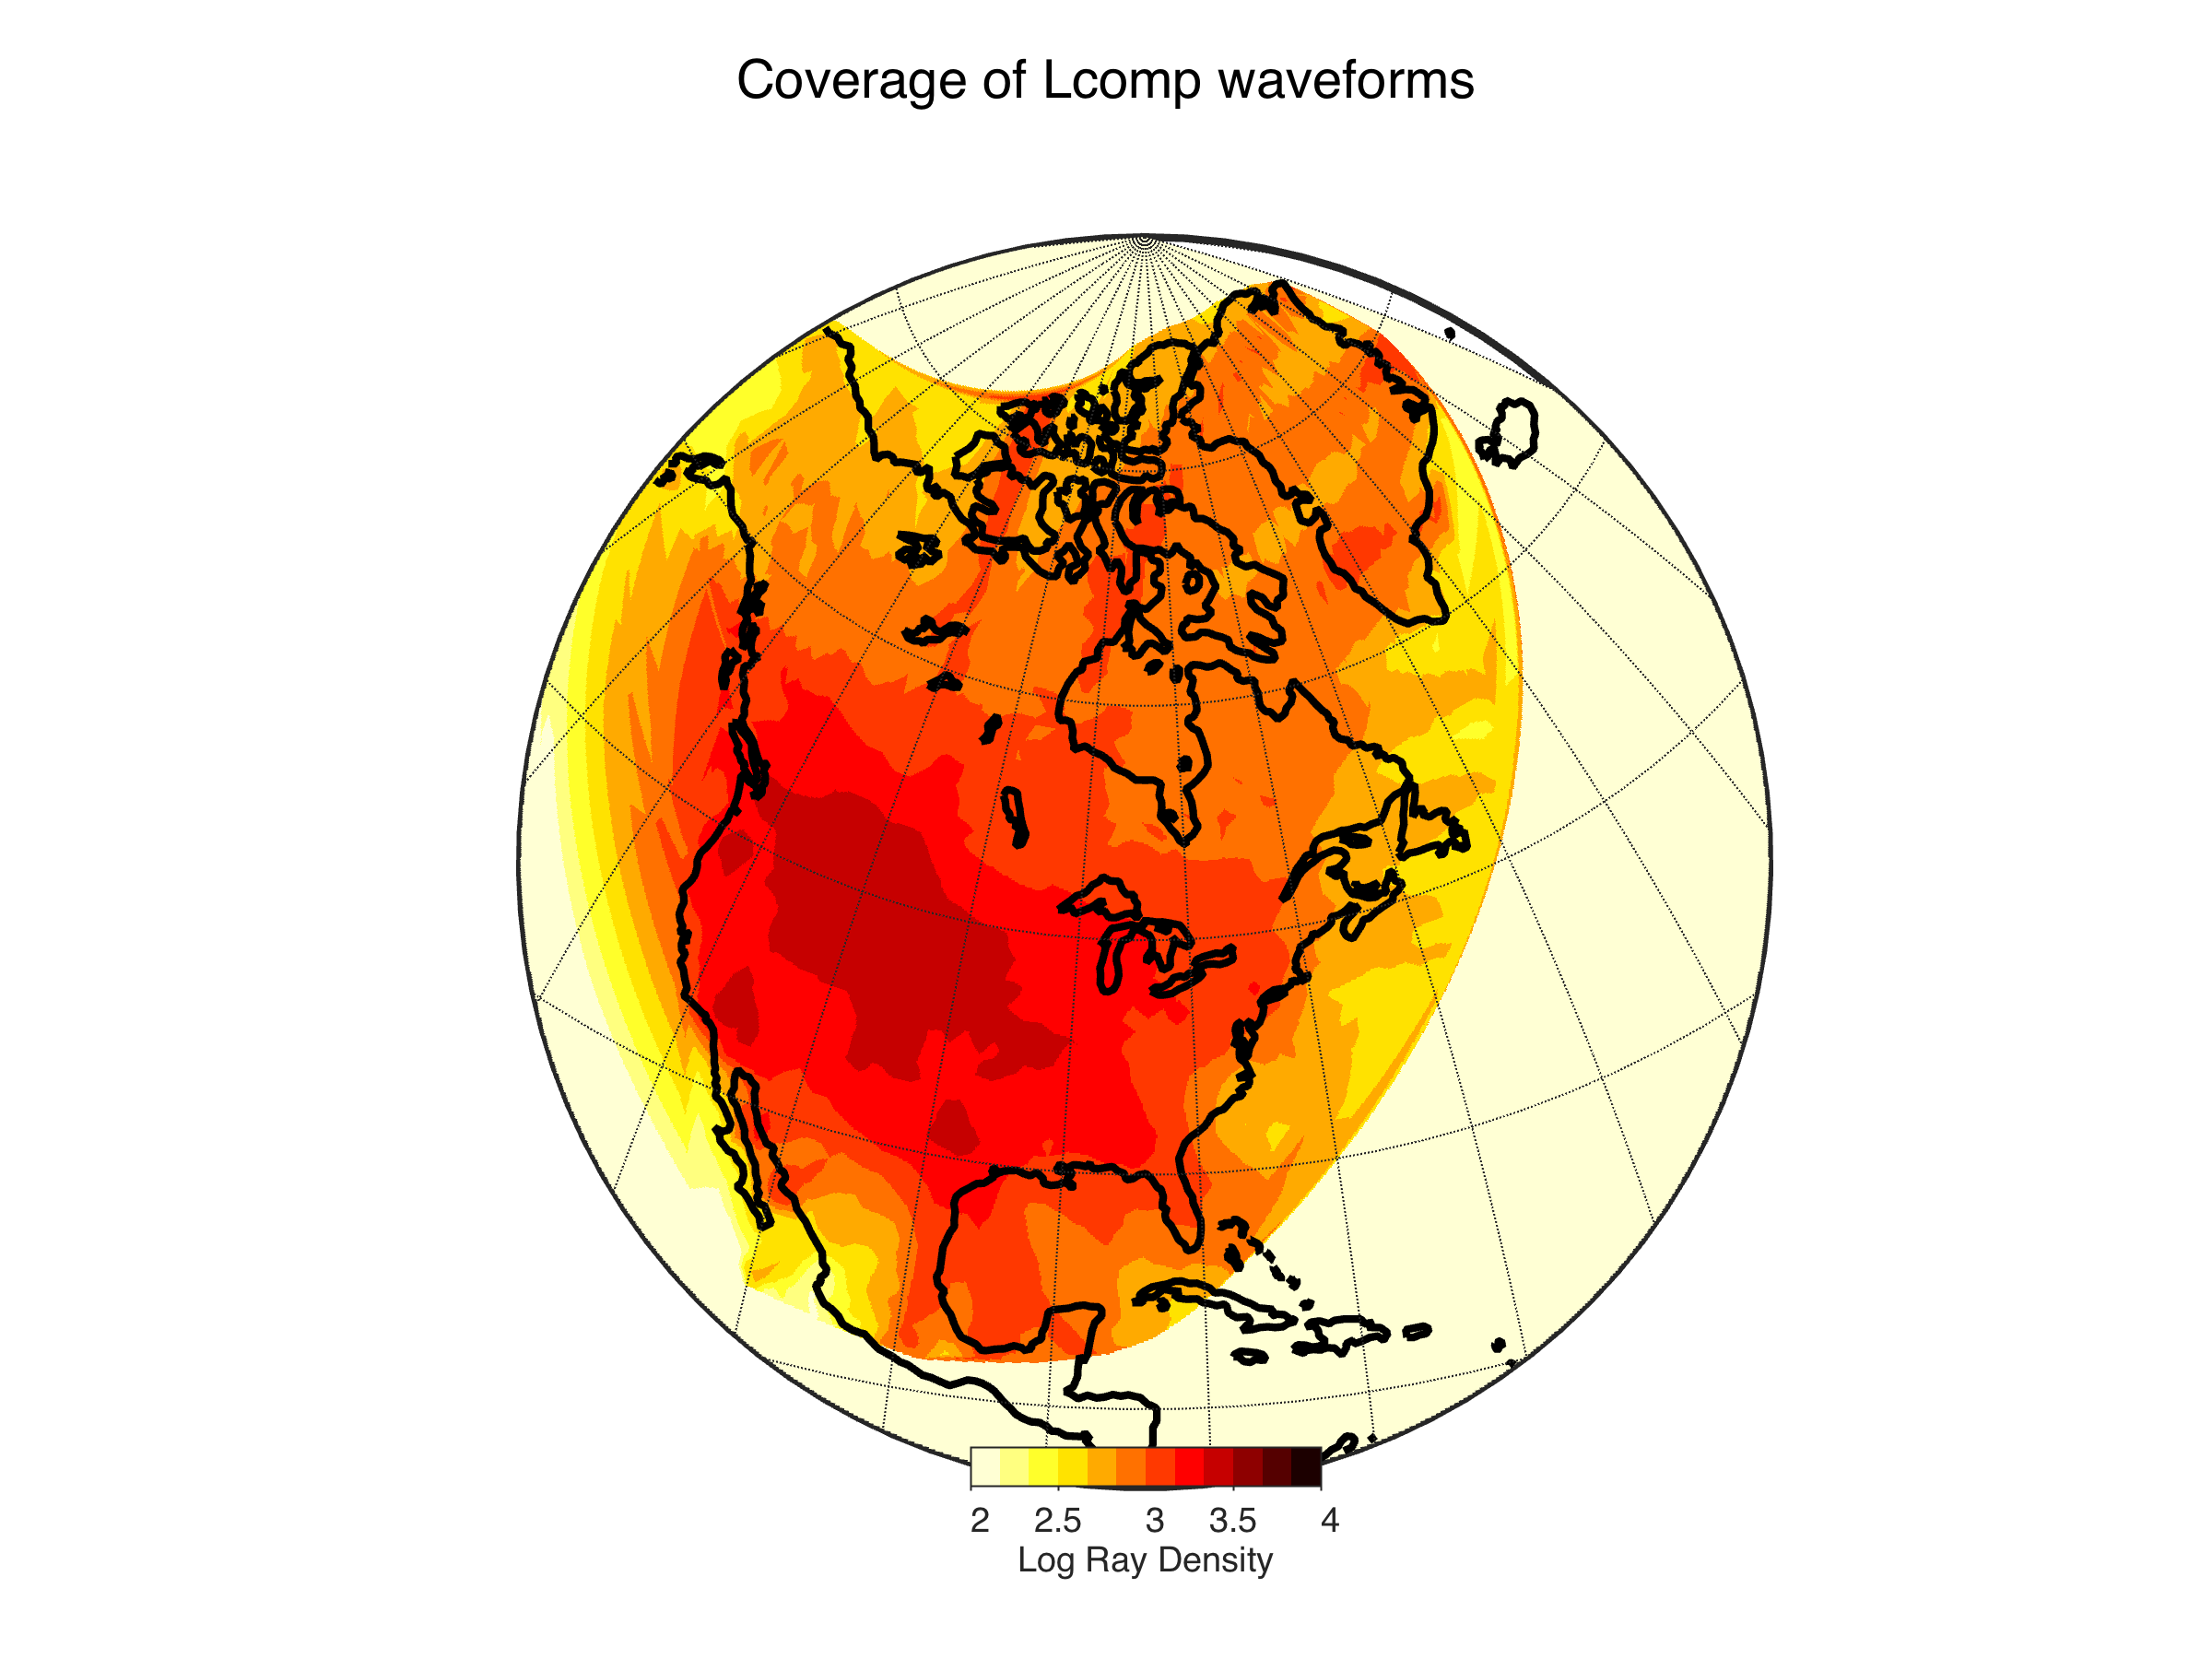
\includegraphics[viewport=120 10 470 420,clip=,width=\linewidth]{figures/Coverage_L_iter3.png}}
		\end{minipage}
		\hfill
		\begin{minipage}{0.47\linewidth}
			\centerline{\includegraphics[viewport=120 10 470 420,clip=,width=\linewidth]{figures/Coverage_T_iter3.png}}
		\end{minipage}

		\begin{minipage}{0.47\linewidth}
			\centerline{\includegraphics[viewport=120 10 470 420,clip=,width=\linewidth]{figures/Coverage_Z_iter3.png}}
		\end{minipage}
		\hfill
		\begin{minipage}{0.47\linewidth}
			\centerline{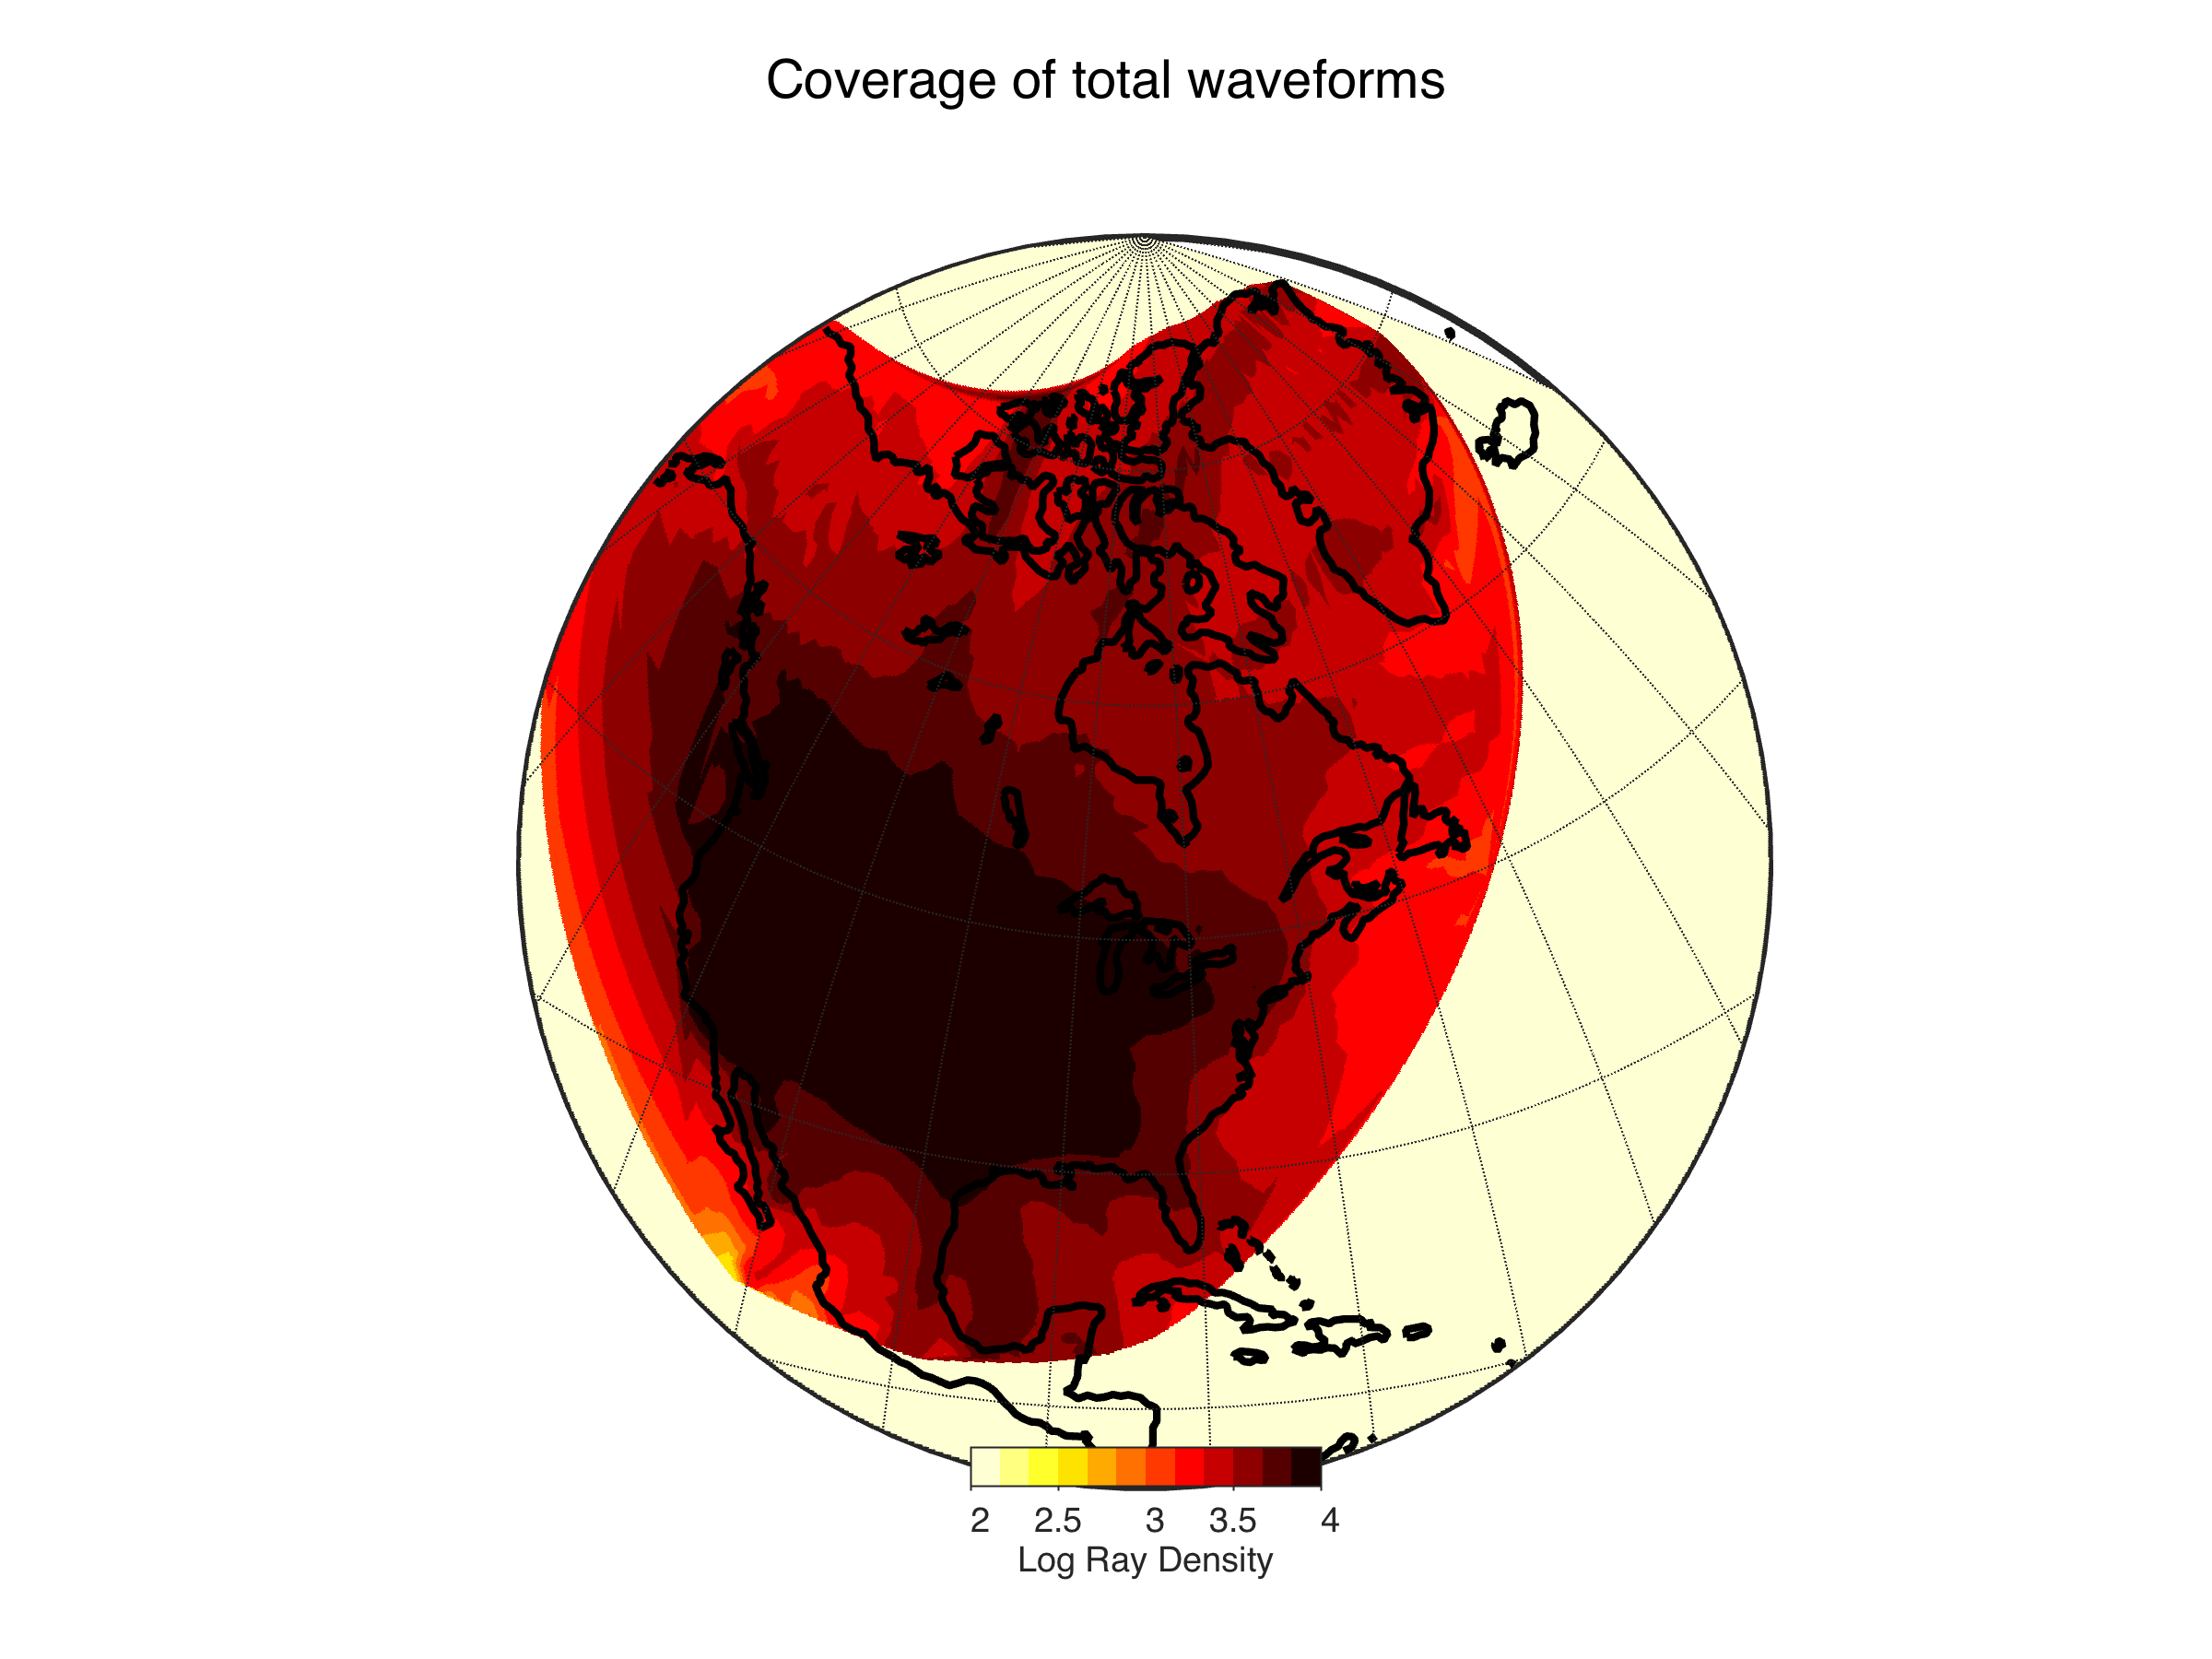
\includegraphics[viewport=120 10 470 420,clip=,width=\linewidth]{figures/Coverage_all_iter3.png}}
		\end{minipage}

		\caption{Density coverage for each component and all gathered.} 
		\label{density_coverage}

	\end{figure}


	% Box Tomo
	\begin{figure}
		\begin{tabular}{ccc}
			(a)&&(b)\\
			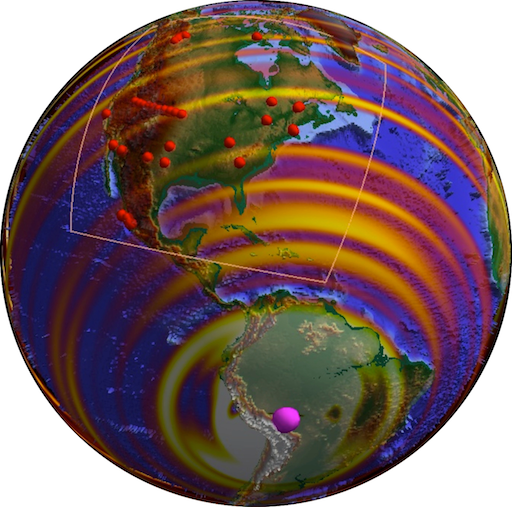
\includegraphics[width=.4\textwidth]{figures/snap_glob.pdf} && 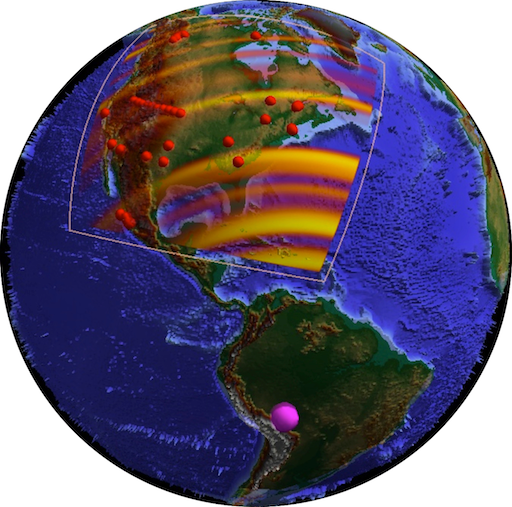
\includegraphics[width=.4\textwidth]{figures/snap_reg.pdf} \\ 
			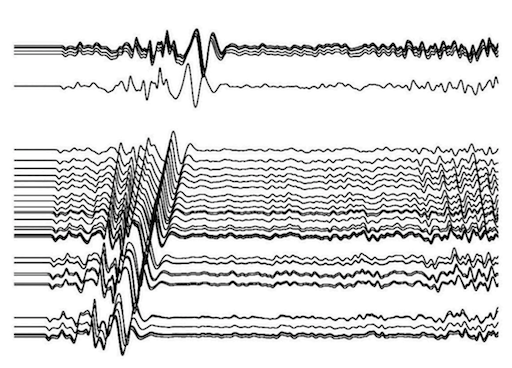
\includegraphics[width=.4\textwidth]{figures/seismo.pdf}    && 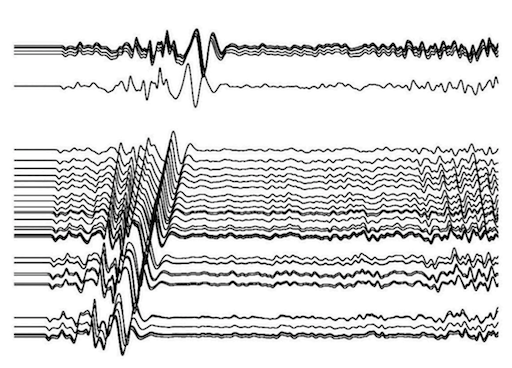
\includegraphics[width=.4\textwidth]{figures/seismo.pdf}
		\end{tabular}

		\caption{\baselineskip 18pt 
			Comparison between a global scale simulation and a regional scale simulation of wave propagation following an earthquake in south America. The seismograms corresponds to the recordings at 37 station located in north America (red spheres).
			The pink sphere shows the epicenter of the earthquake. In (a), the wavefield is modeled globally using the spectral element method Specfem3D\_globe \citep{komatitsch2002spectrala}. In (b), the wavefield is modeled regionally using the RegSEM. During the inversion, all the synthetic seismograms are computed using the regional SEM code RegSEM \citep{cupillard2012regsem} code and regenerated thanks to virtual sources located around the computational domain \citep[see][]{masson2013numerical}. The sismograms in (b) are exactly similar to those in (a), however, the computational effort is greatly reduced in the regional simulation (b).}

		\label{injection}

	\end{figure}

	 % 3d map of Vs
	\begin{figure}
		\centering
		\includegraphics[width=1\textwidth]{figures/Vs-60-300-for-paper.png}

		\caption{\baselineskip 18pt
		3D isotropic shear wave velocity structure of the continent. Map views are shown from 60 km down to 300 km, as variations with respect to the regional mean (thick red line in Figure ~\ref{1daverage}) as $\frac{dV_S}{V_{S_{O}}}$ . 
		Below each map, depth and its regional shear velocity mean is indicated. Minimum and maximum perturbations are also indicated.
		}

		\label{3d-VS}

	\end{figure}

	% 3d map of Xi
	\begin{figure}
		\centering
		\includegraphics[width=1\textwidth]{figures/Xi-60-300-for-paper.png}

		\caption{\baselineskip 18pt
		3D radial anisotropic structure of the continent. Map views are shown from 60 km down to 300 km, as variations with respect to the regional mean (thick red line in Figure ~\ref{1daverage}) as $\frac{d\xi}{\xi_{O}}$ . 
		Below each map, depth and its regional shear velocity mean is indicated. Minimum and maximum perturbations are also indicated.
		}

		\label{3d-Xi}

	\end{figure}

	% 1D profiles
	\begin{figure}
		\centering
		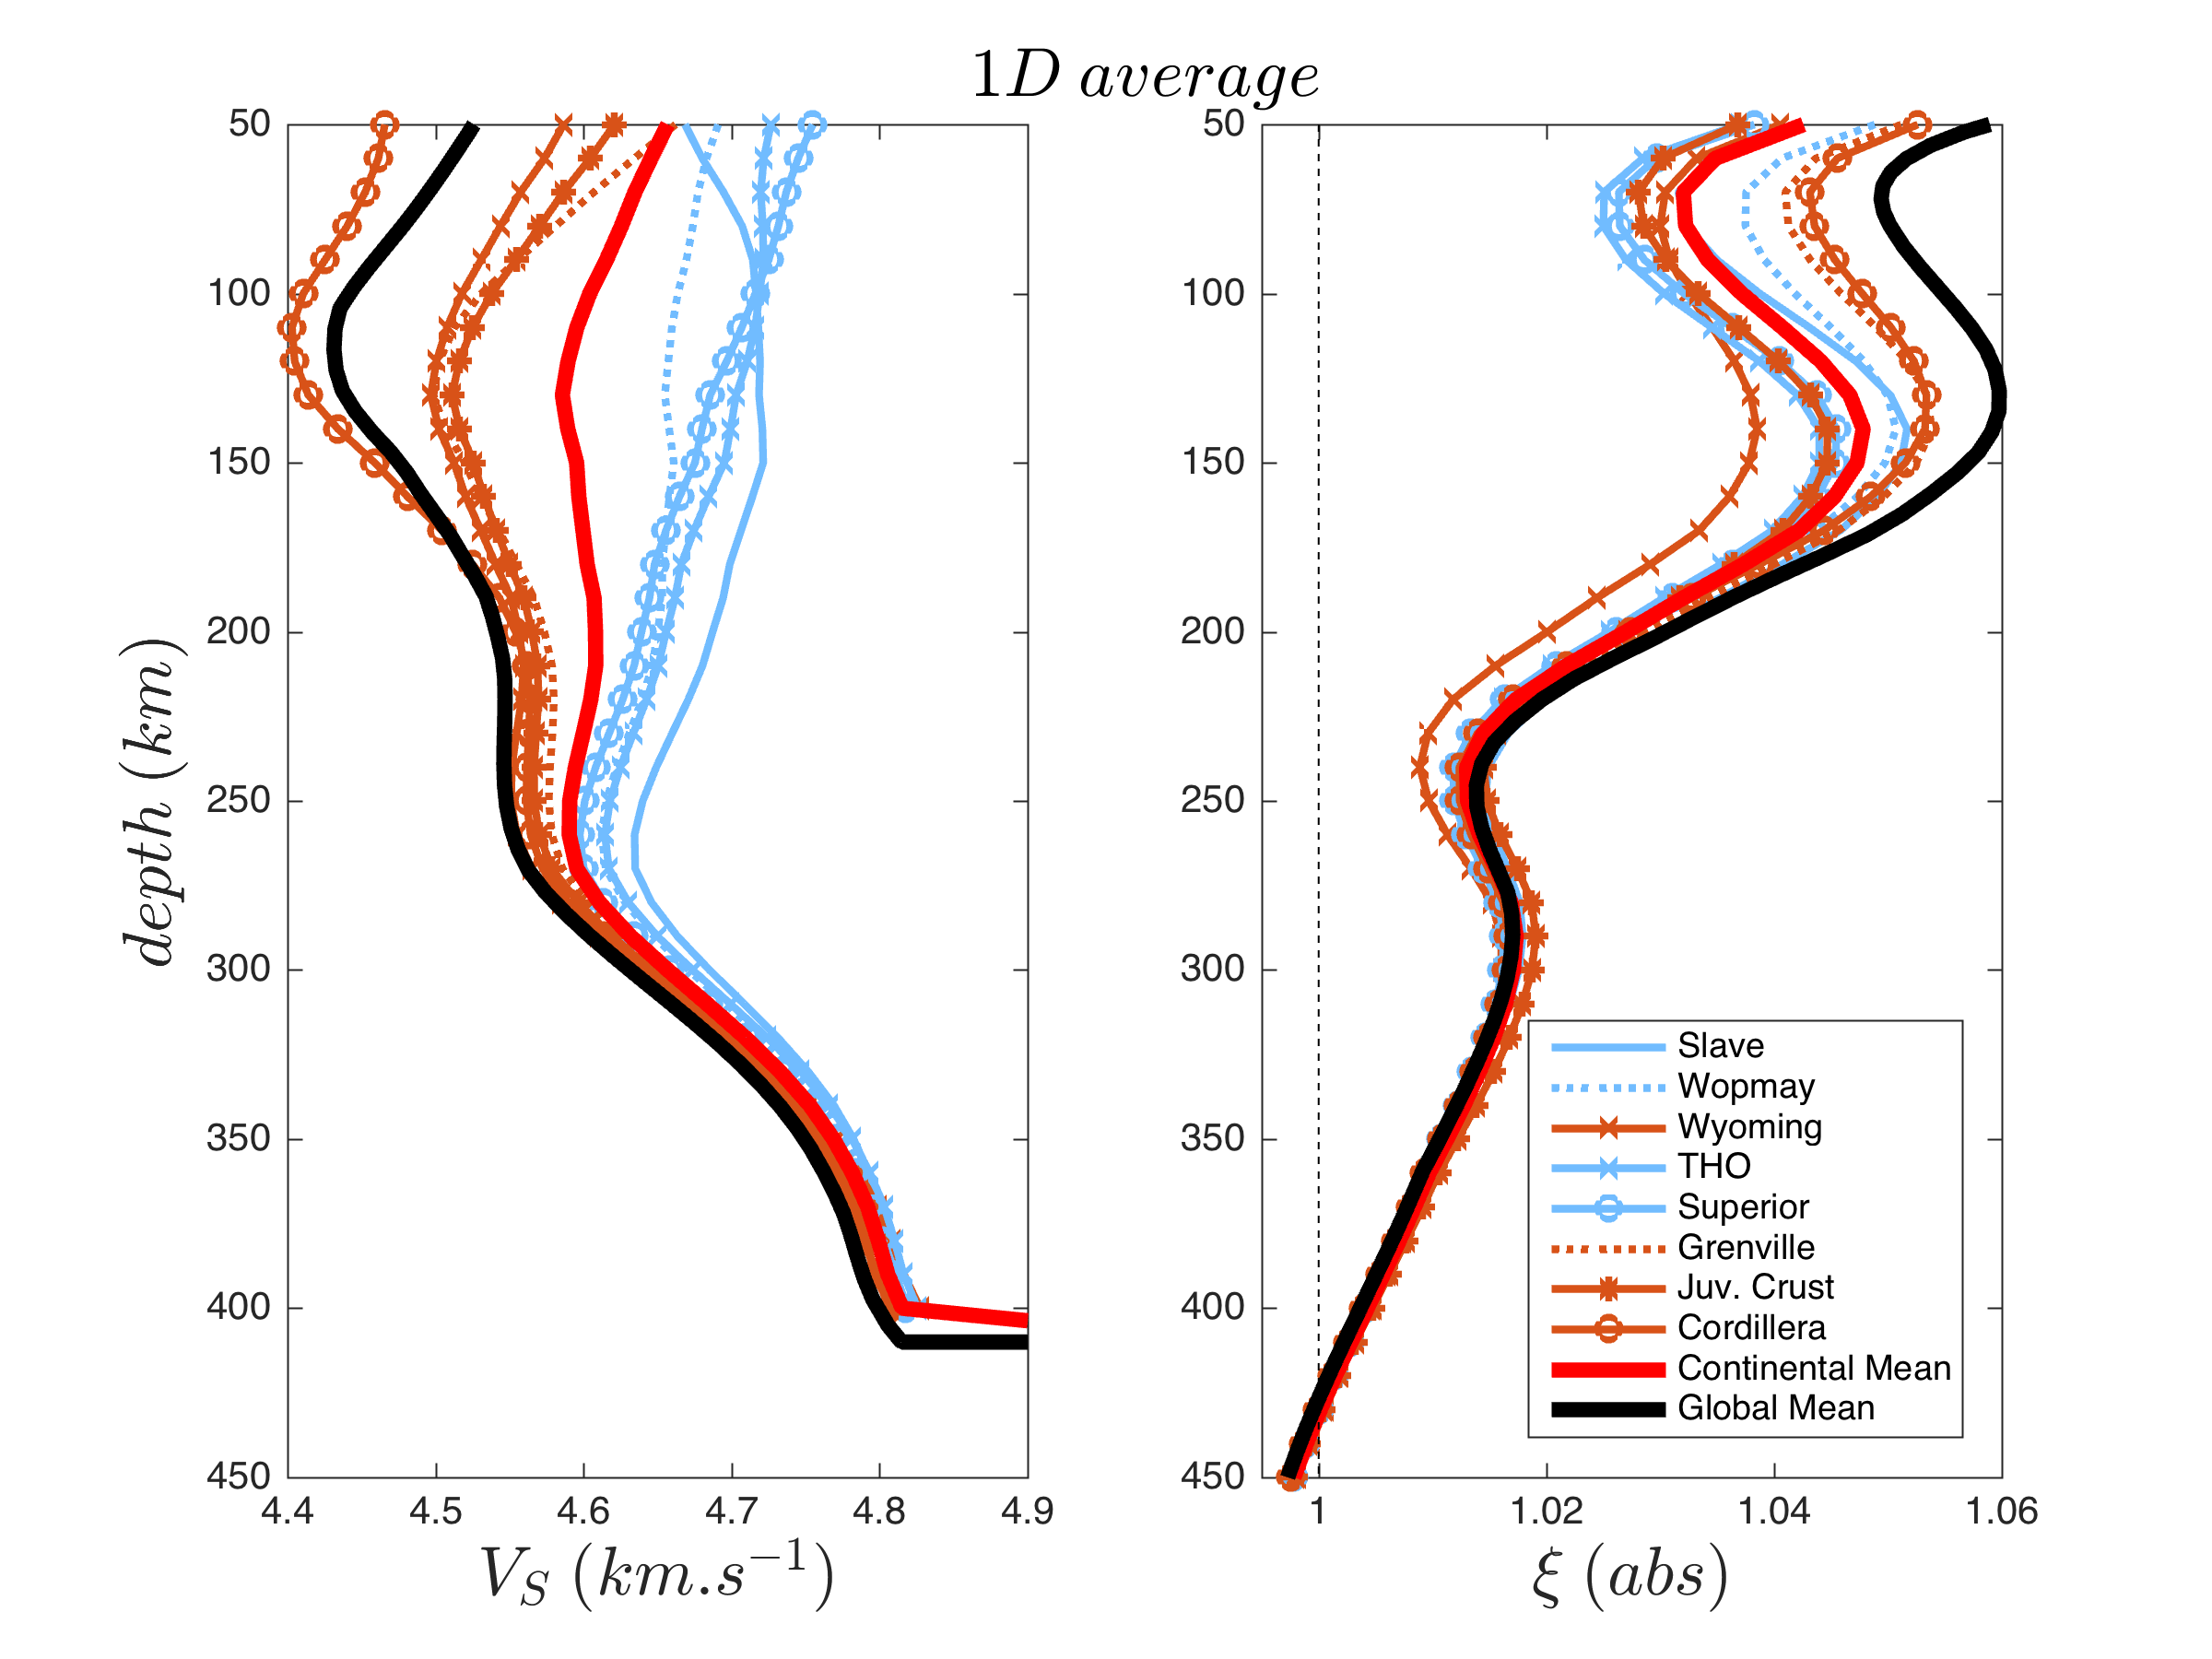
\includegraphics[width=1\textwidth]{figures/1D_profile_with_regions.png}

		\caption{\baselineskip 18pt 
		1D average depth profiles for isotropic shear velocity (left) and radial anisotropy (right), for the SEMucb\_wm1 global model (thick black), the continental average (thick red); and depth profiles for different regions in the model (see legend and Figure~\ref{mapgeol}). The continental average is always higher than the global average in terms of $V_S$, while for $\xi$, they are similar deeper than $250 \: km$.}
		\label{1daverage}
	\end{figure}

	% Xsections of the craton
	\begin{figure}
		\begin{minipage}{0.5\linewidth}
			\centerline{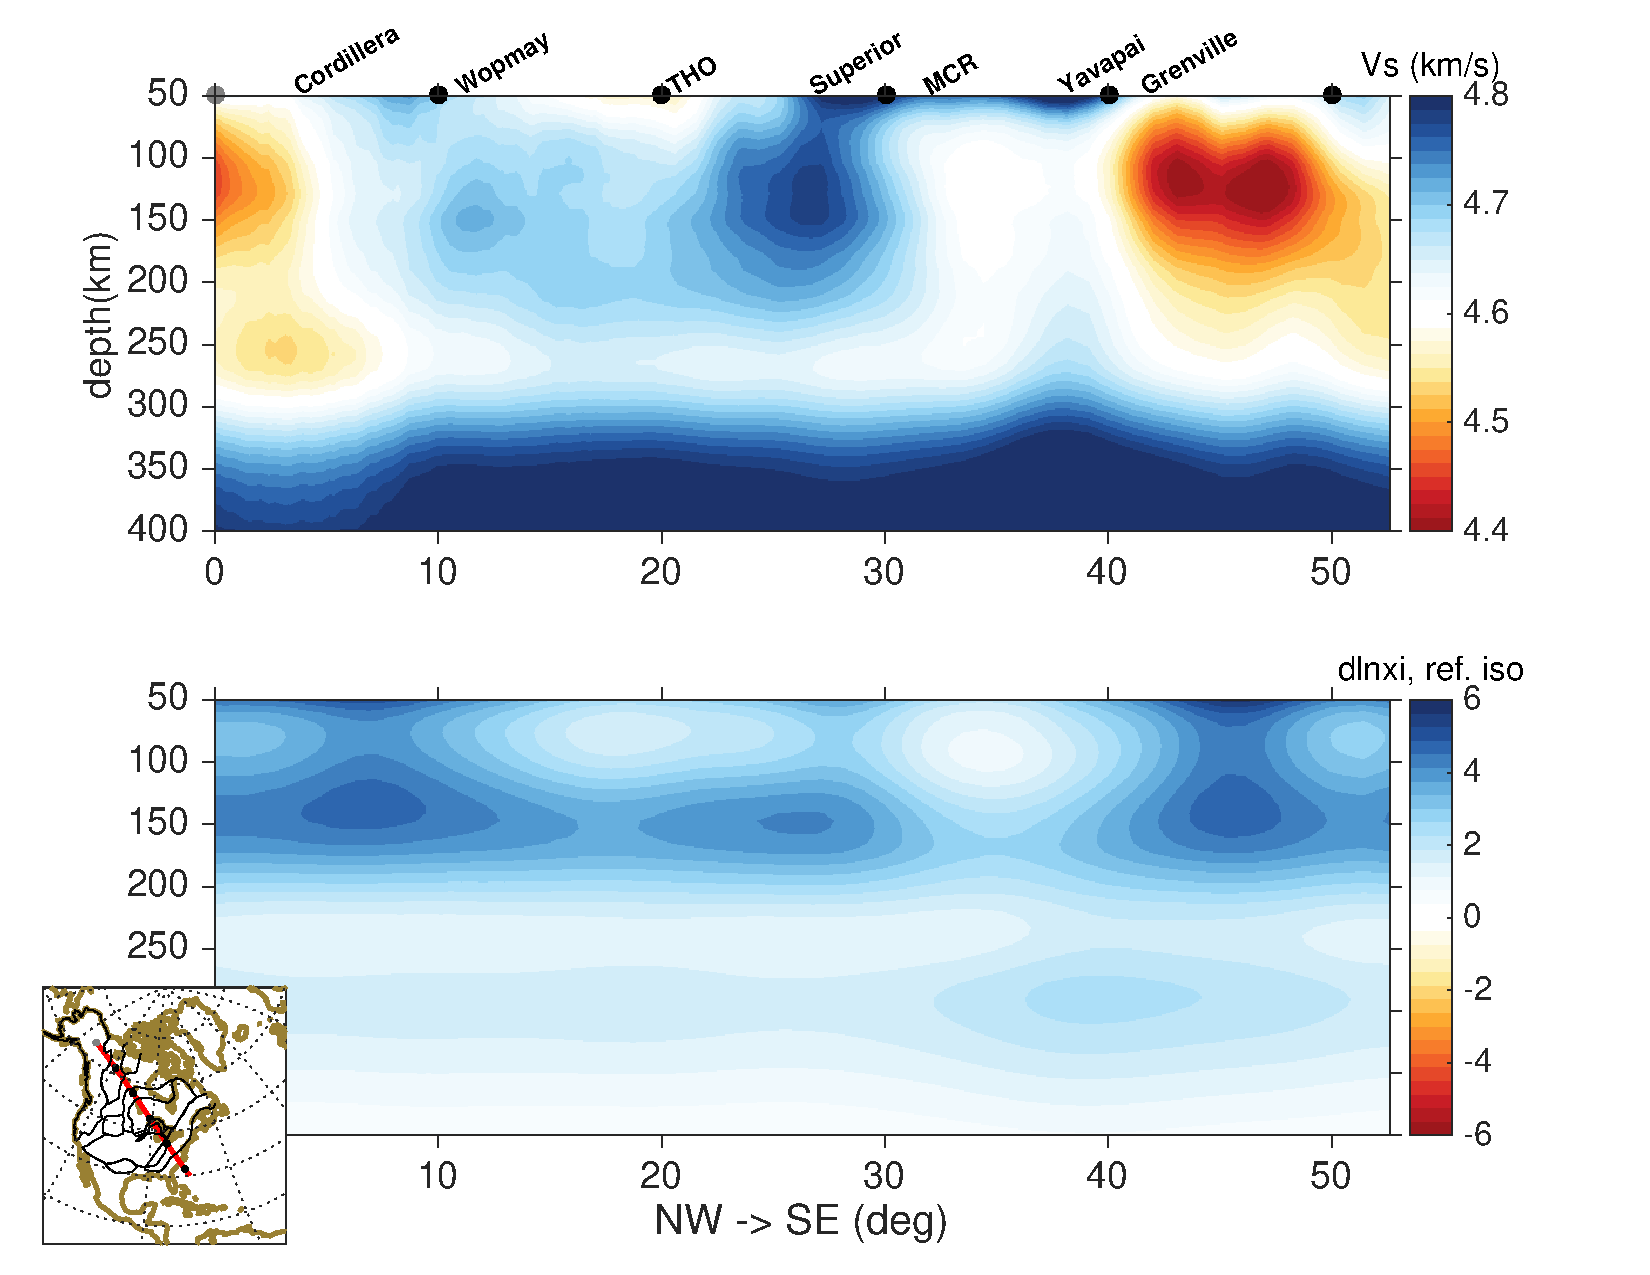
\includegraphics[width=\linewidth]{figures/profiles_NASEM3_vs_dxi_A.pdf}}
		\end{minipage}
		\hfill
		\begin{minipage}{0.5\linewidth}
			\centerline{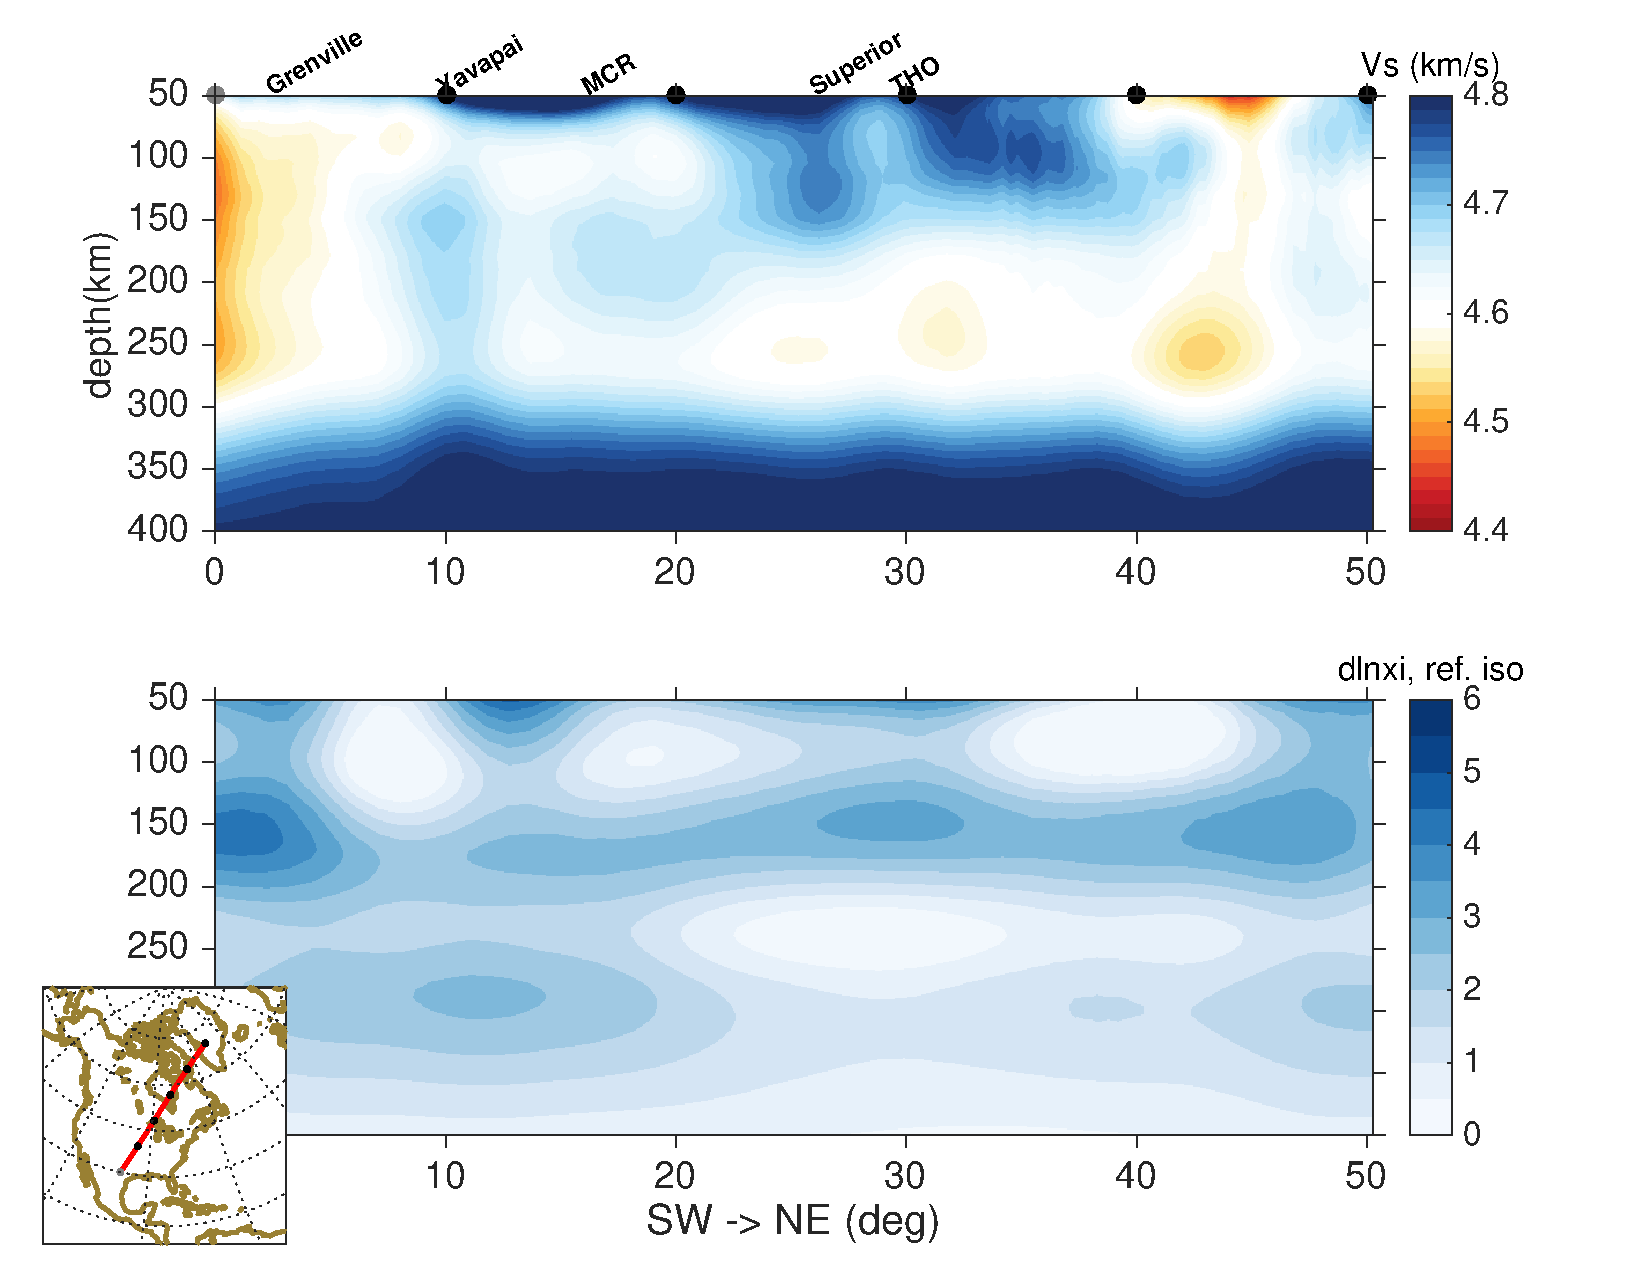
\includegraphics[width=\linewidth]{figures/profiles_NASEM3_vs_dxi_B.pdf}}
		\end{minipage}

		\caption{Cross Section of the lithospheric core}
		\label{cratoncross}

	\end{figure}

	\begin{figure}
		\begin{minipage}{0.5\linewidth}
			\centerline{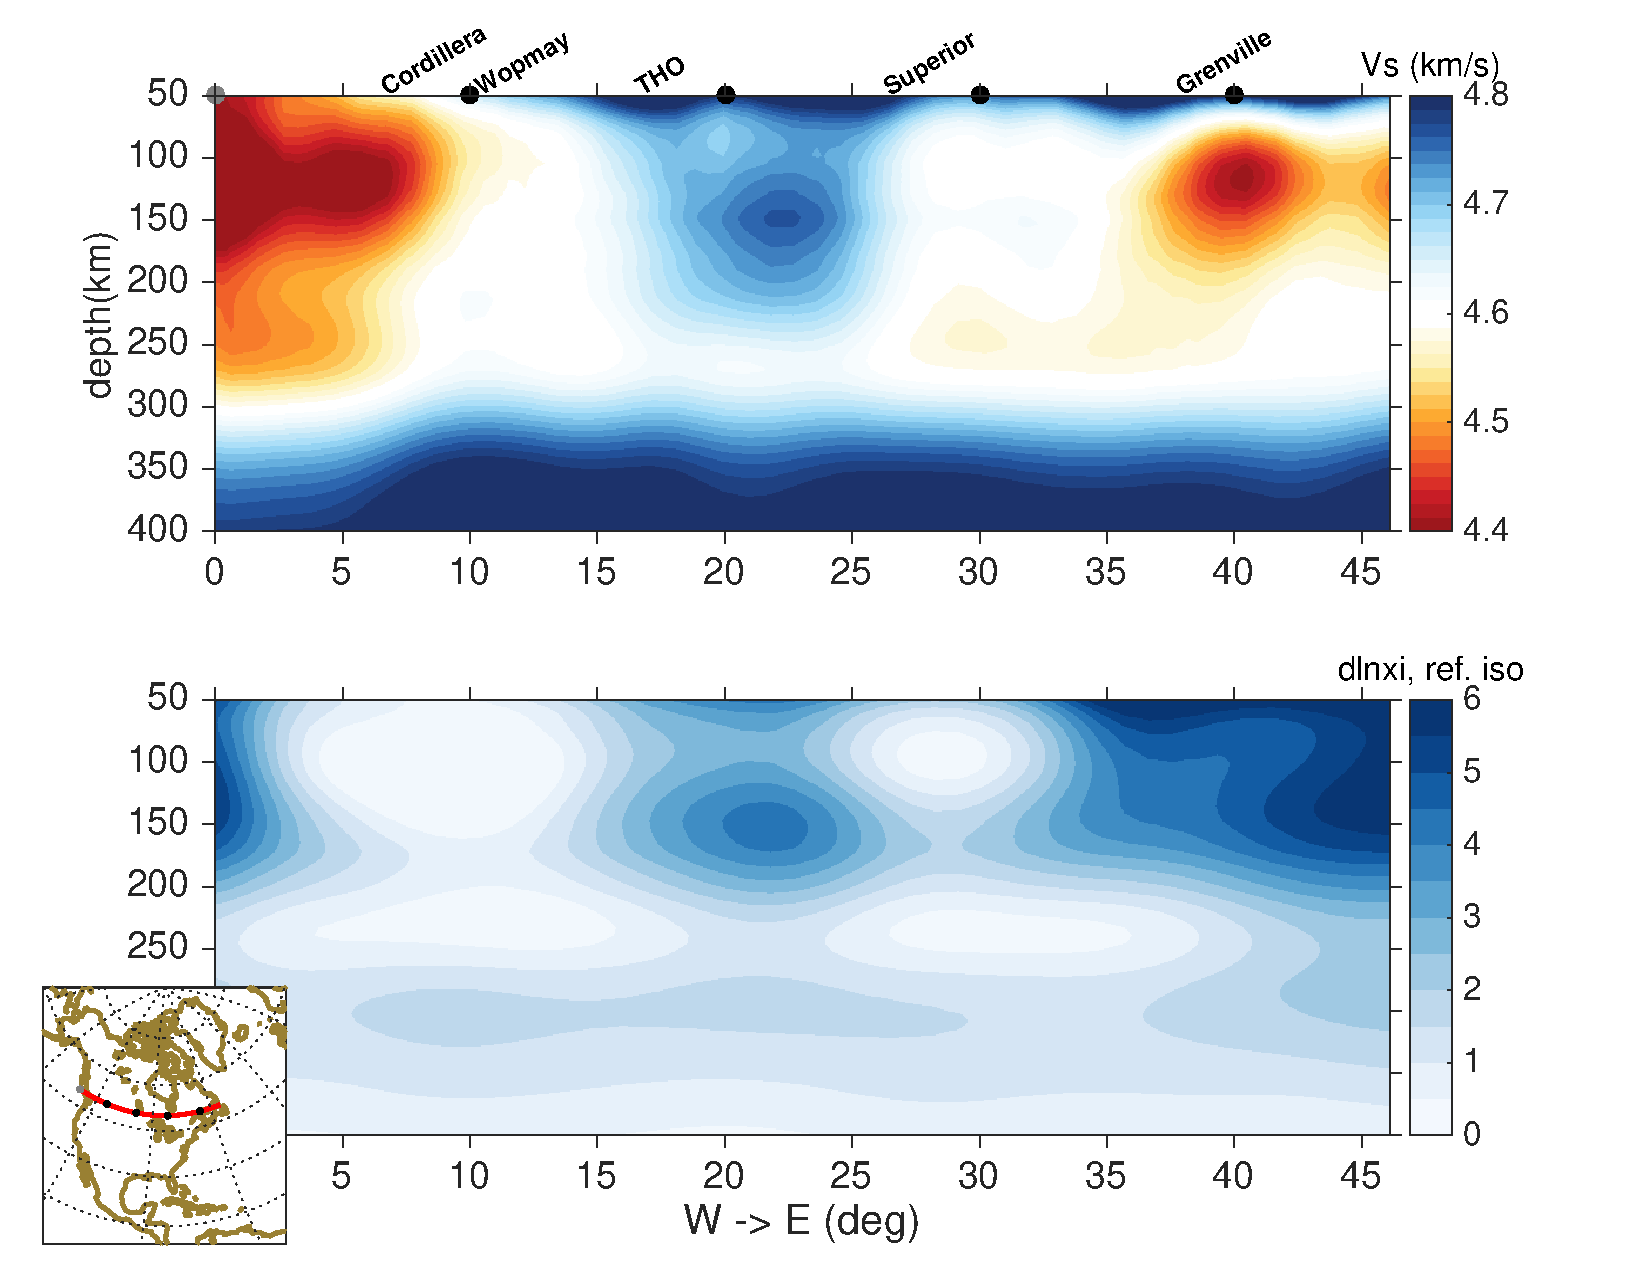
\includegraphics[width=\linewidth]{figures/profiles_WE-50.pdf}}
		\end{minipage}
		\hfill
		\begin{minipage}{0.5\linewidth}
			\centerline{\includegraphics[width=\linewidth]{figures/profiles_SN-100.pdf}}
		\end{minipage}

		\caption{Cross Section of the lithospheric core showing the core retraction}
		\label{cratoncrossedge}

	\end{figure}

	% Xsection of the GMT track
	\begin{figure}
		\centerline{\includegraphics[width=\linewidth]{figures/profiles_NASEM3_vs_dxi_GMTrack.pdf}}

		\caption{Cross Section of the lithosphere along the Great Meteor track based on \cite{heaman2000timing} construction}
		\label{gmtcross}

	\end{figure}

	% dIso for Xi
	\begin{figure}
		\begin{minipage}{0.5\linewidth}
			\centerline{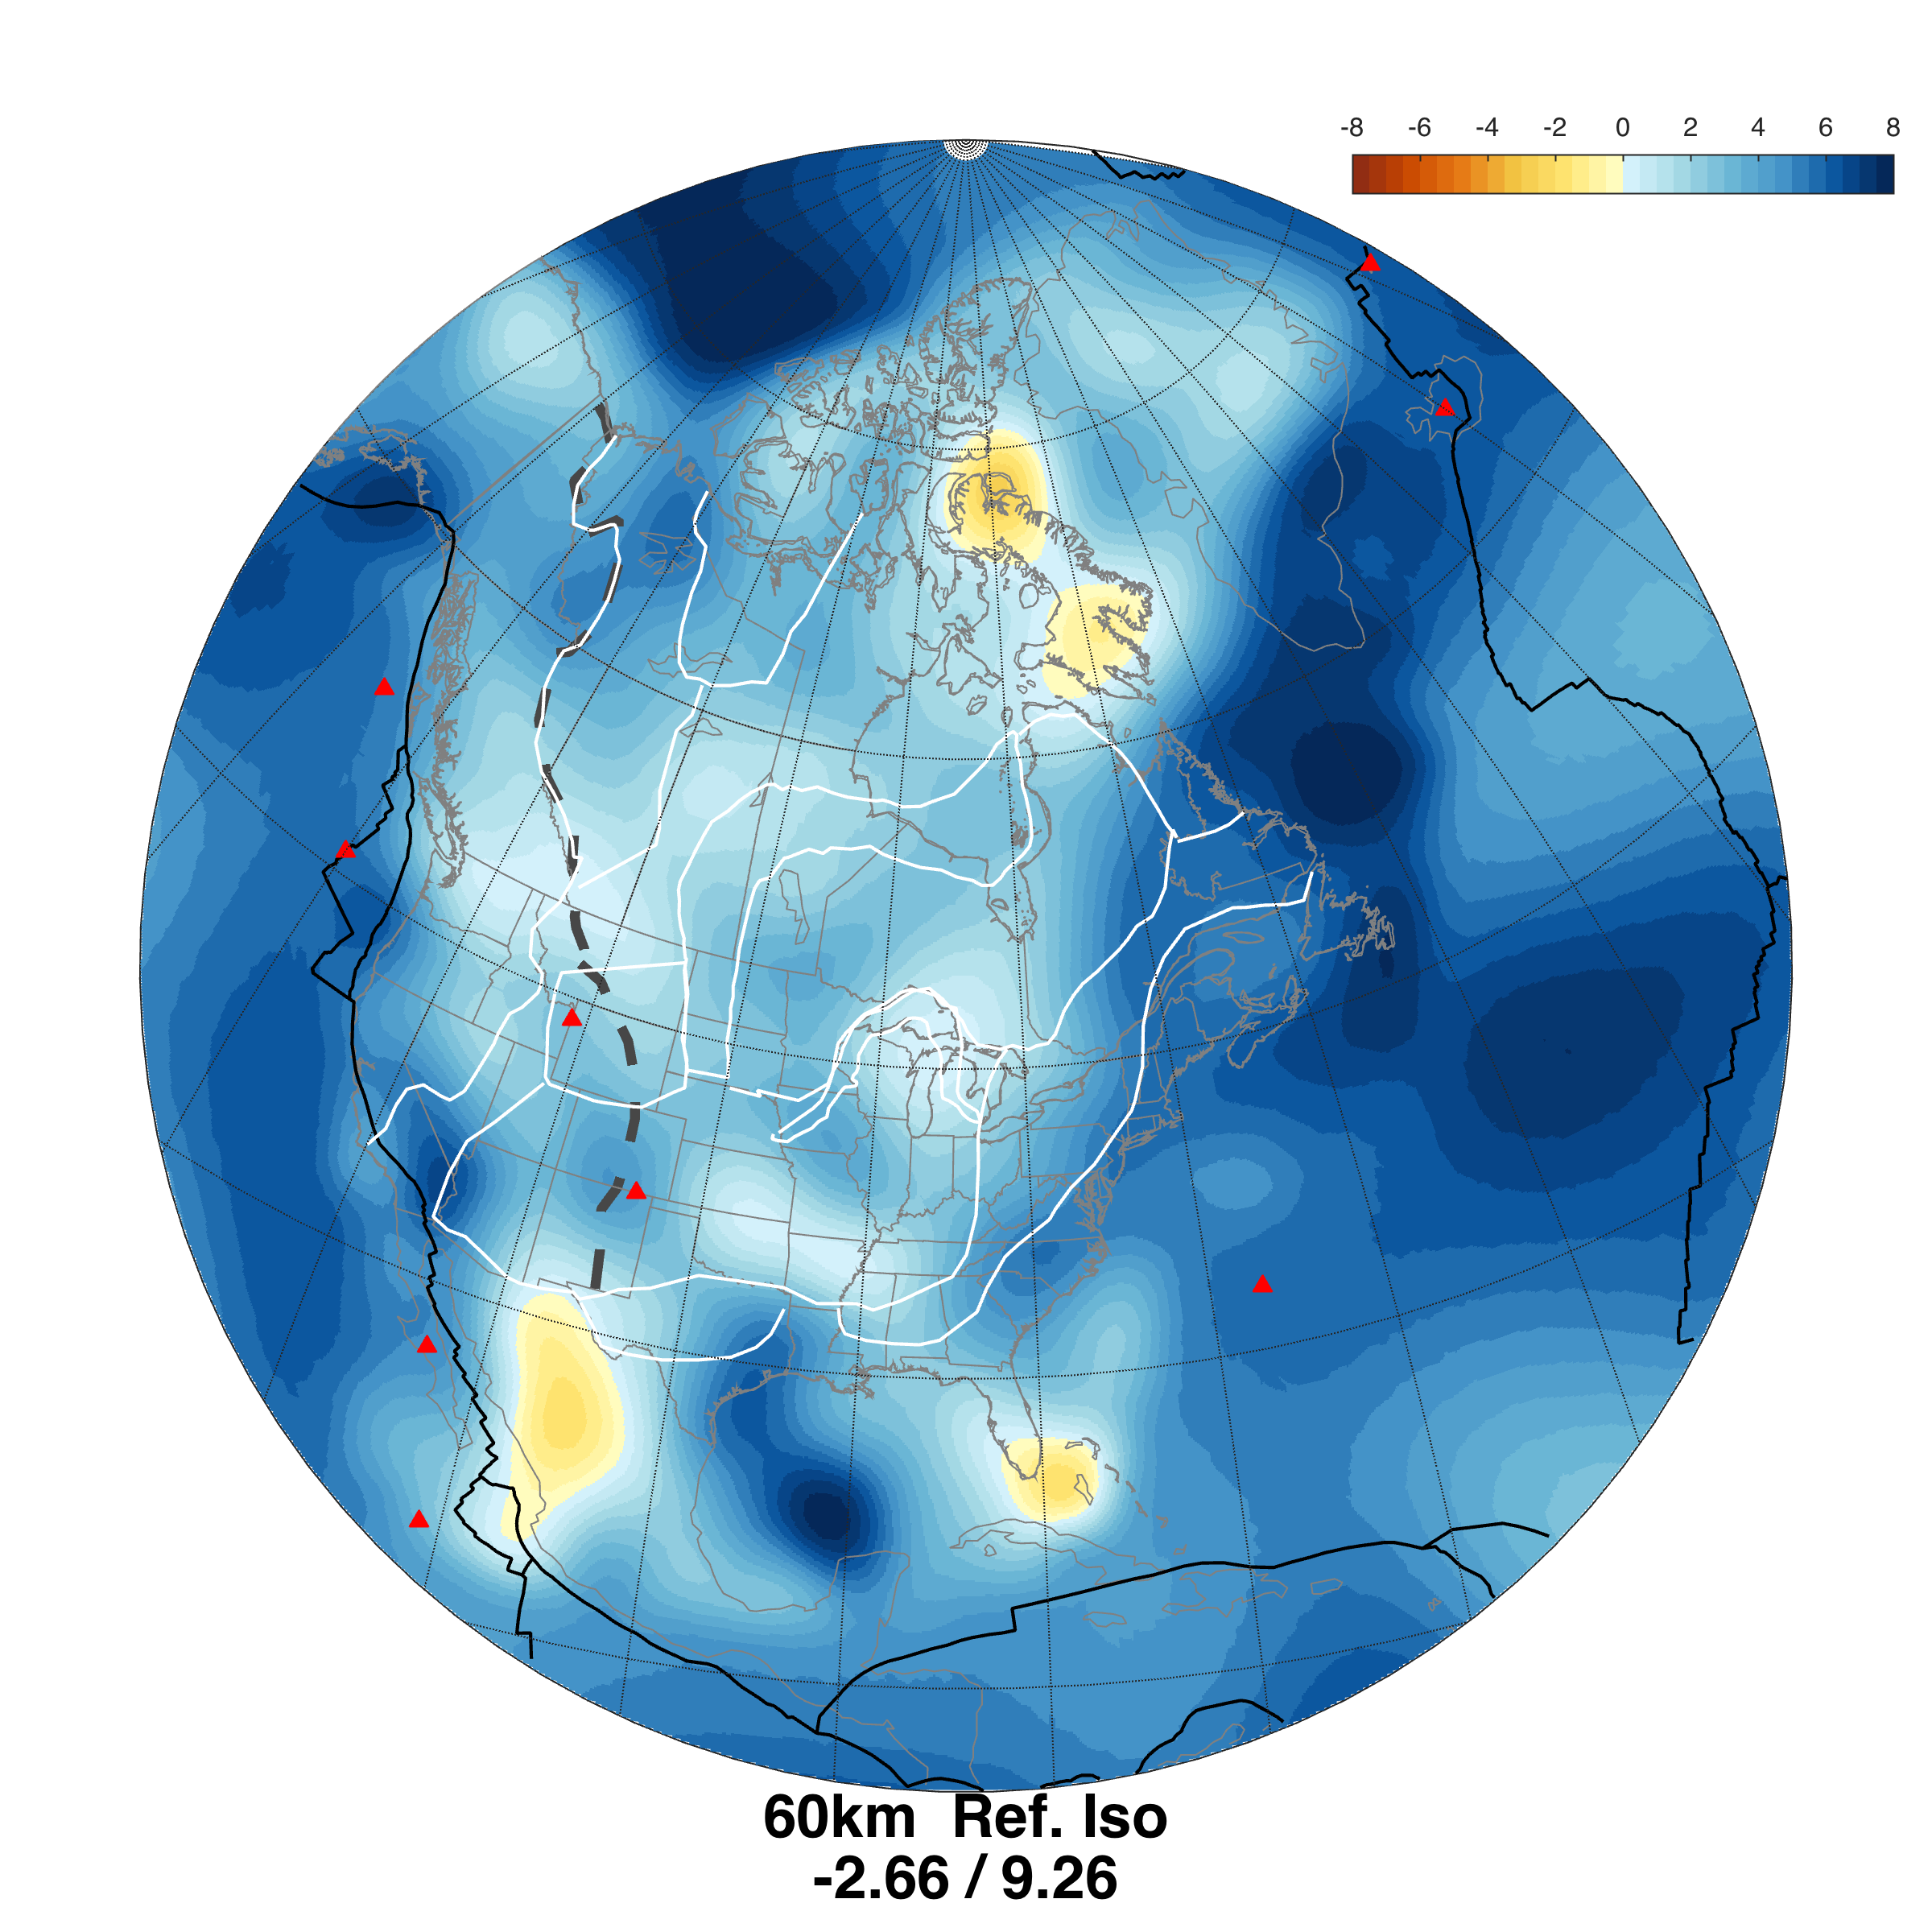
\includegraphics[width=\linewidth]{figures/Xi_NASEM-iter3-Xi-iso_60km.png}}
		\end{minipage}
		\hfill
		\begin{minipage}{0.5\linewidth}
			\centerline{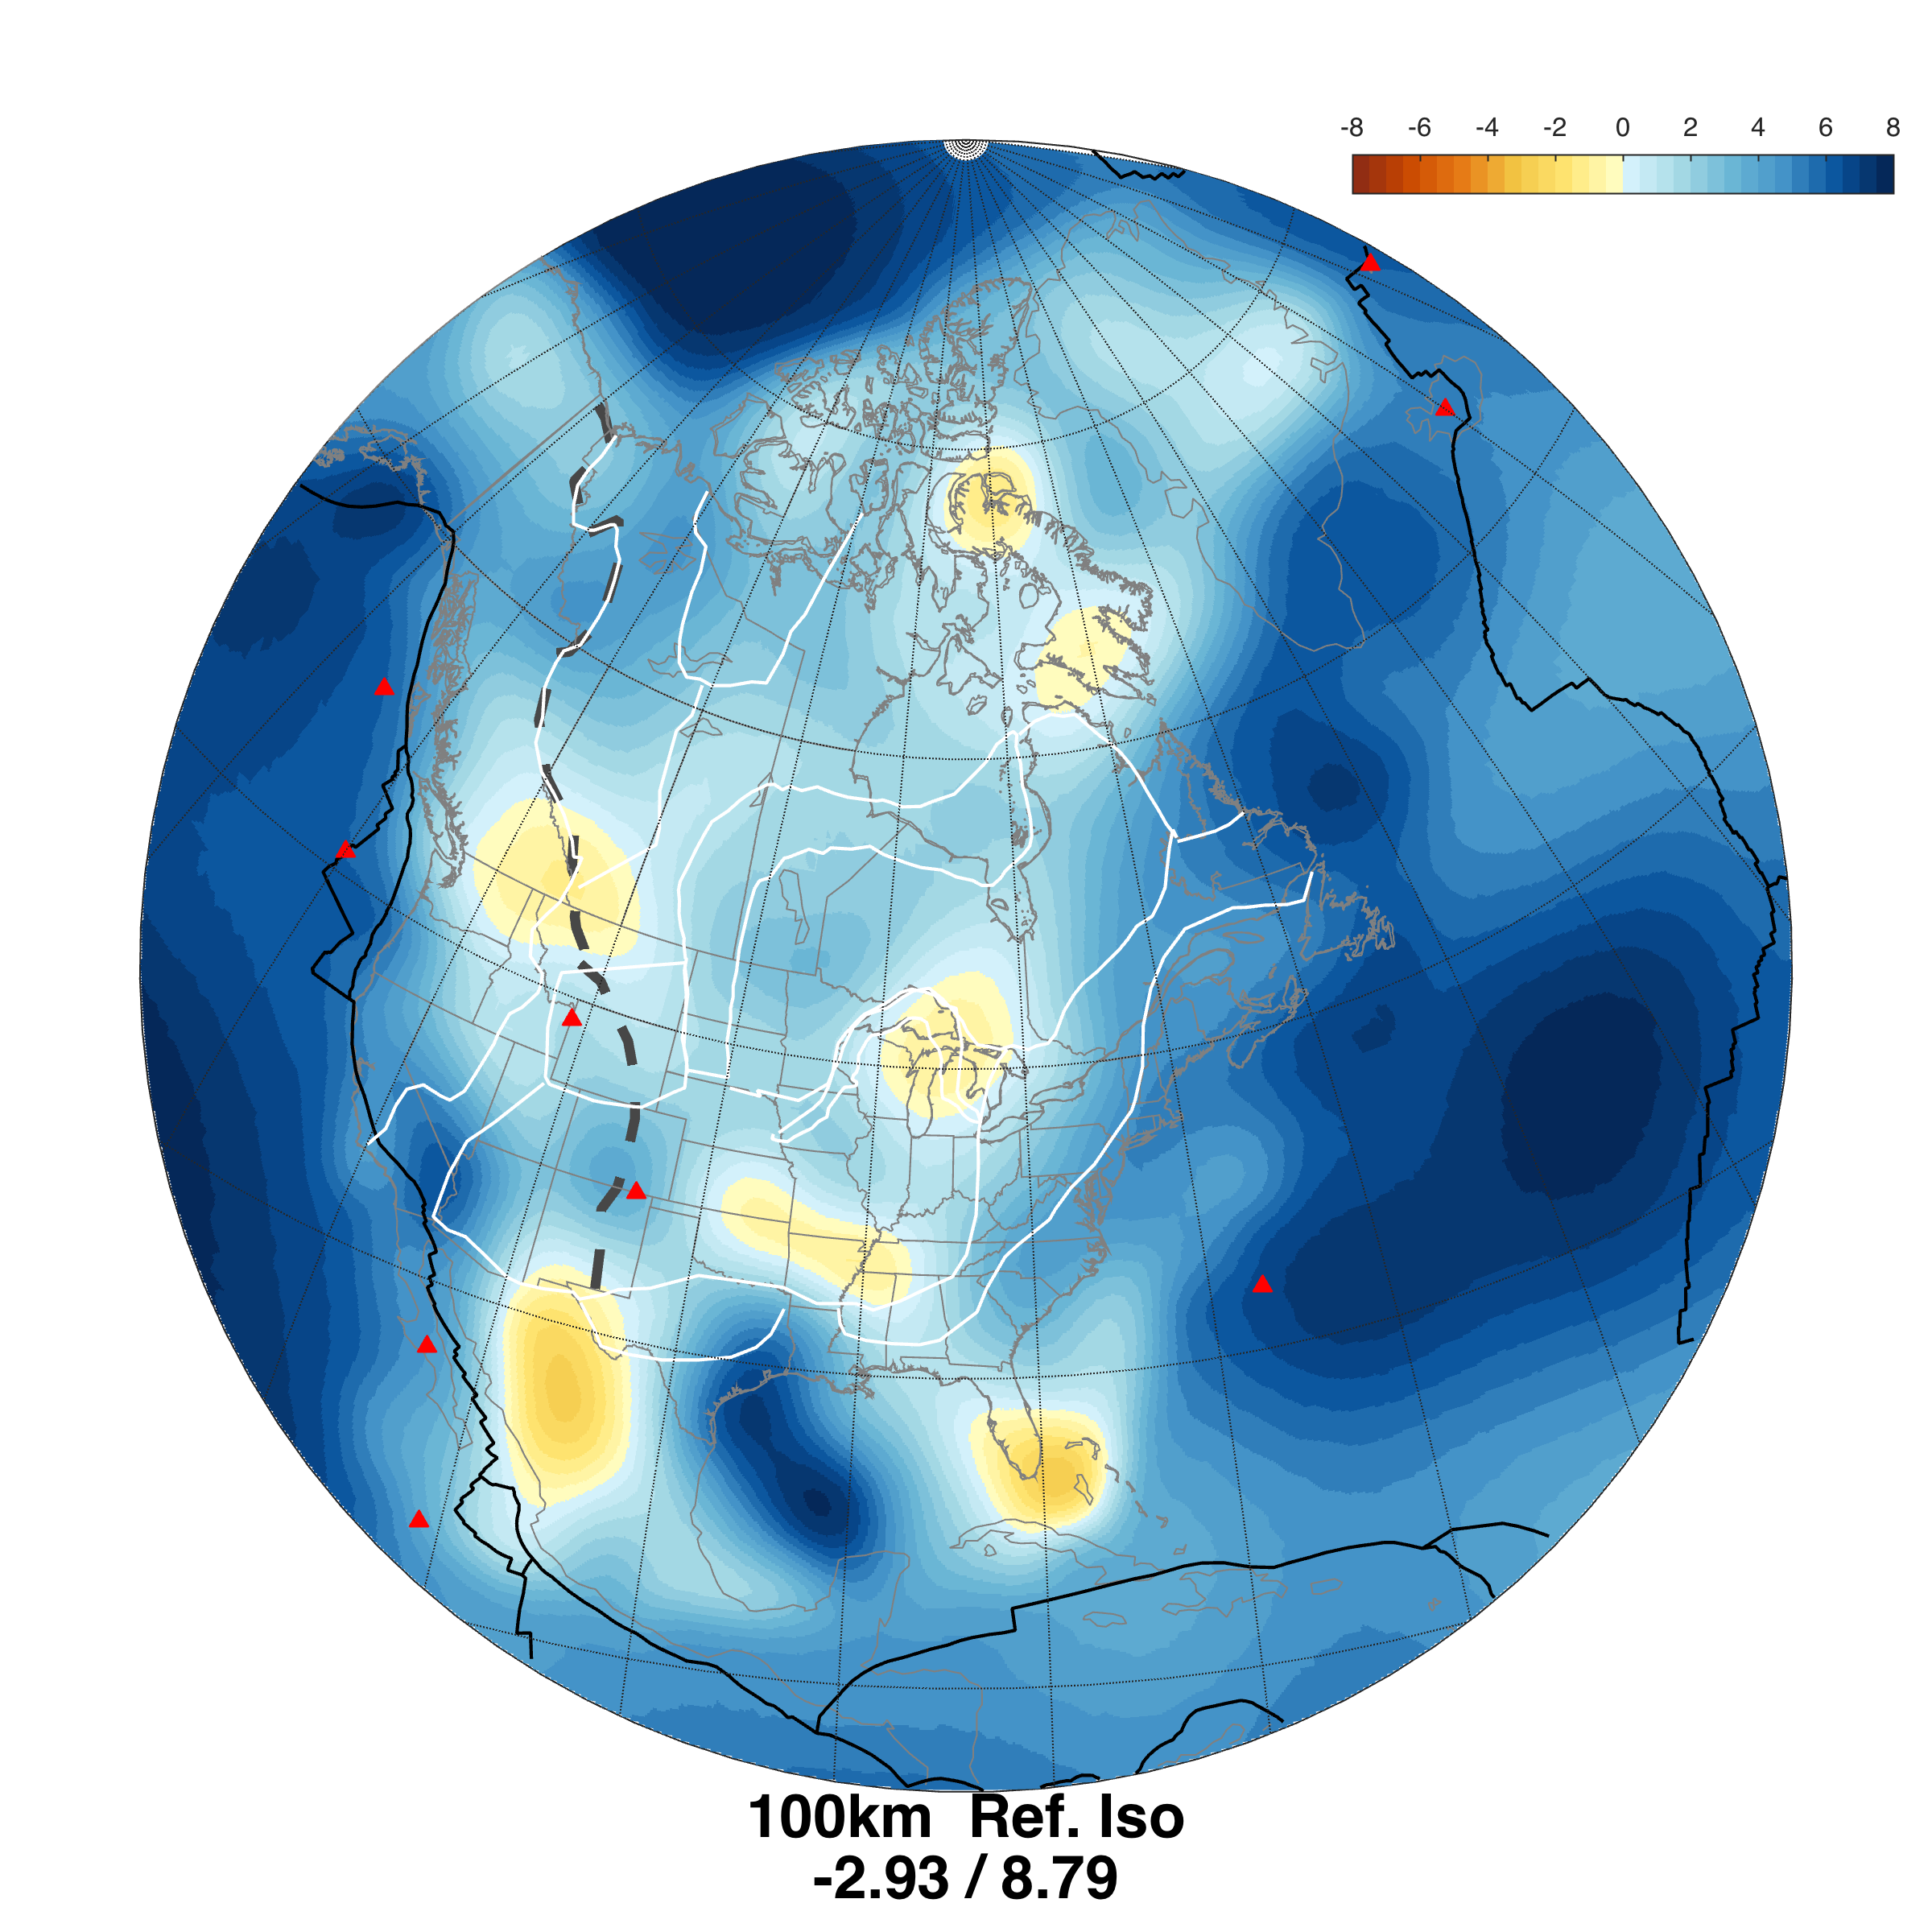
\includegraphics[width=\linewidth]{figures/Xi_NASEM-iter3-Xi-iso_100km.png}}
		\end{minipage}
		% \begin{minipage}{0.5\linewidth}
		% 	\centerline{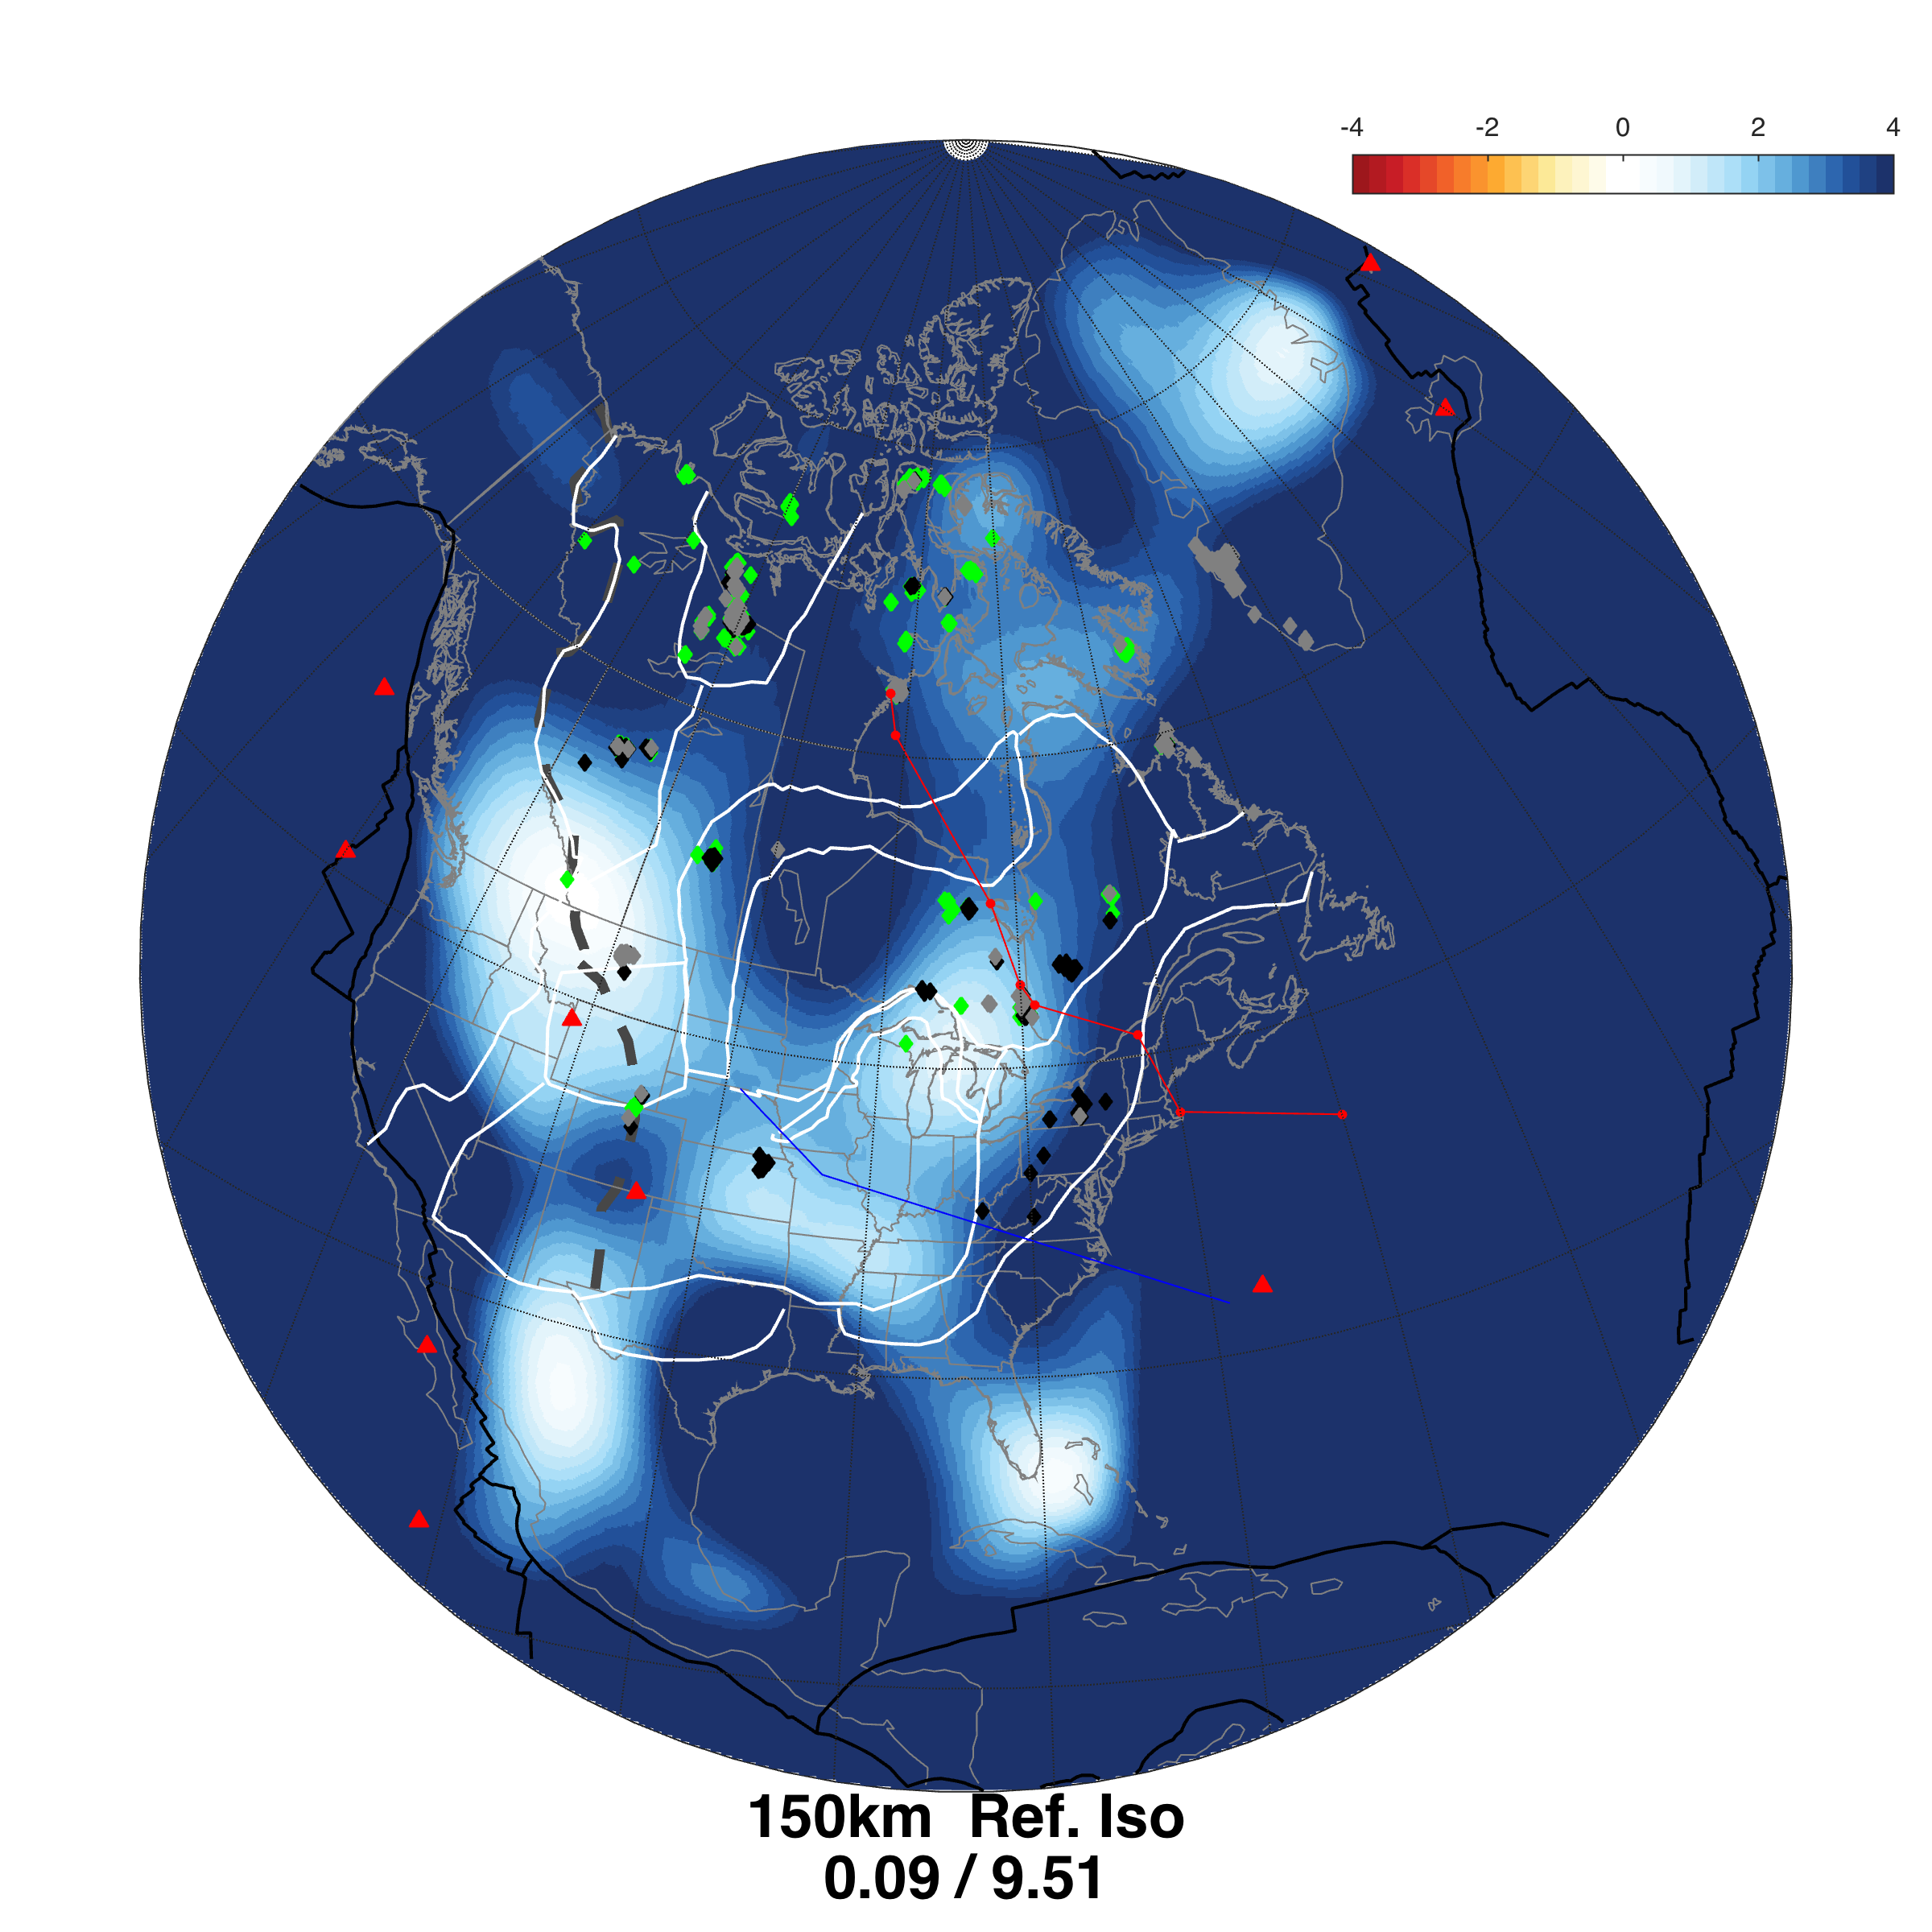
\includegraphics[width=\linewidth]{figures/Xi_NASEM-iter3-Xi-iso_150km.png}}
		% \end{minipage}

		\caption{\baselineskip 18pt 
		3D radial anisotropic structure of the continent at 60 and 100 \: km compared to the Isotropic case. 
		Map view shows variations with respect to the Isotropic case as $\frac{\xi - 1}{1}$ in \%. 
		Map view is saturated to better show where $V_{SV}$ is stronger than $V_{SH}$.
		Below each map, depth and its regional shear velocity mean is indicated. Minimum and maximum perturbations are also indicated.}
		\label{3d-xi-iso-100km}

	\end{figure}
\bibliographystyle{apalike}
\bibliography{/Users/Pierre/Documents/PHD/Thesis/biblio.bib}
%
\end{document}

%